
\color{black}

\chapter{Эвиденциальность и <<перфектоиды>> в нарративах} \label{sec:intro3}

Как отмечено в \citep{labovwaletzky1967}, по сравнению с обычной речью в нарративах говорящие пользуются более ограниченным набором глагольных форм. Говорящие выбирают  определенную форму для главной линии рассказа, а другие формы играют вспомогательную роль для внутреннего структурирования текста или оформления фоновых событий и дополнительных сведений. Для главной линии наиболее характерны перфективные формы глагола или пунктивные предикаты, поскольку они обозначают законченные действия и тем самым имплицируют возможность какого-то последующего действия, тогда как у имперфективных и дуративных форм, которые соответственно употребляются для оформления фоновых событий и информации, эта возможность отсутствует \citep{hopper1982}. Особые эффекты употребления форм несовершенного вида, в частности, форм настоящего времени, в нарративе обсуждаются в \citep[287-290]{paducheva2010}. Согласно Р. Шинжато, употребление в фоновых эпизодах свойственно и эвиденциальным перфектоидам, например, старояпонской форме со вспомогательным глаголом \textit{-keri}, по контрасту с \textit{-ki} образующим нечто наподобие аориста \citep{shinzato1991}. По мнению Шинзато, это связано с исходными, видо-временным значением перфекта, который обозначает дуративное событие. Хотя эвиденциальный перфектоид, в отличие от прототипического перфекта, также встречается в главной линии нарратива, такое употребление считается диагностикой для <<неперфектности>>, как уже обсуждалось в разделе \ref{sec:pftyp}. Внутри главной линии чередование разных форм может структурировать дискурс. В саларском языке тюркской семьи формы прямой засвидетельствованности в незасвидетельствованном нарративе, который в целом основан на использовании заглазных форм, используются для выдвижения какого-то события на передний план \citep[55--56]{dwyer2000}, см. подробнее о разного рода отступлениях от основной линии в разделе \ref{sec:methodanalysis}. В любом случае, в нарративах одна форма как правило преобладает над другими.
\par В цезском языке нахско-дагестанской семьи, где оппозиция прямой и косвенной засвидетельствованности считается грамматикализованной (см., однако, обсуждение в \ref{sec:direct}), говорящие могут употреблять форму прямой засвидетельствованности в заглазном нарративе для <<приближения>> рассказа к моменту речи и его участникам, аналогично употреблению форм настоящего времени в рассказах о прошлом \citep{comriepolinsky2007}. В приложении к статье Комри и Полинской приводится история на диалекте с. Кидеро, в которой рассказчик начинает рассказывать в прошедшем заглазном, после чего переключается на прошедшее очевидное, хотя речь идет о легендарных событиях. Там же отмечается, что форму глагола в первом предложении можно было бы рассматривать как нарративное обрамление, после которого допускается переключение на форму с очевидным значением допускается. Тем не менее в течение рассказа говорящий несколько раз возвращается к прошедшему заглазному, и мотивация этих переключений остается не до конца понятной, на что указывает Д. Форкер \citep[499]{forker2018evid}. Возможно, здесь играет роль функция внутреннего структурирования дискурса, хотя моменты переключения в цезском тексте не маркируют явные переходы на фоновые события. Это подтверждается и тем, что почти во всех случаях одну форму можно заменить другой \citep[342--343]{comriepolinsky2007}. В нахско-дагестанских языках мы находим разные нарративные стратегии. Кроме стратегии с общим прошедшим, в нарративах о незасвидетельствованных событиях отмечается упомянутая выше стратегия с заглазным перфектоидом, а также стратегии с репортативом и с особым вспомогательным глаголом в роли показателя эвиденциальности. Отдельной стратегией можно считать случаи, в которых рассказ начинается с эвиденциально маркированной формы, после чего рассказчик переходит на менее маркированную форму (например, общее прошедшее). В зависимости от режима повествования встречаются стратегии, перечисленные в таблице \ref{tab:narstrats}. По-видимому, контекст прямой засвидетельствованности --- наименее маркирован, и общее прошедшее --- нейтрализующее значение.
Следует иметь в виду, что приведенный нами список стратегий отнюдь не исчерпывающий.

\begin{table}[H]
\caption{Нарративные стратегии в нахско-дагестанских языках}
\label{tab:narstrats}
\vspace{0.1cm}
\begin{center}
\begin{tabular}{lcc}
                                                                                                                           & \begin{tabular}[c]{@{}c@{}}Прямая засв.\end{tabular} & \begin{tabular}[c]{@{}c@{}}Косвенная засв.\end{tabular} \\ \hline
\multicolumn{1}{l|}{Общее прошедшее}                                                                                       & +                                                                        & +                                                                           \\
\multicolumn{1}{l|}{Перфектоид}                                                                                            & -                                                                        & +                                                                           \\
\multicolumn{1}{l|}{Репортативная частица}                                                                                 & -                                                                        & +                                                                           \\
\multicolumn{1}{l|}{Специализированный всп. гл.}                                                                           & -                                                                        & +                                                                           \\
\multicolumn{1}{l|}{\begin{tabular}[c]{@{}l@{}}Обрамление перфектоидом и\\ общее прошедшее в главной\\ линии\end{tabular}} & -                                                                        & +                    
\end{tabular}
\end{center}
\end{table}

Остается неизученным, коррелируют ли разные нарративные стратегии с конкретными жанрами нарратива. Про эвиденциальные показатели известно, что они склонны к конвенционализации в определенных нарративных жанрах --- становятся \textsc{признаками жанра}. В традиционных повествовательных жанрах, таких как сказки, и особенно в сказочных формулах, употребление показателя часто зависит не от говорящего и его источника информации, а от условностей нарративных традиций. Во многих языках такую роль играют репортативные показатели. В нахско-дагестанских языках, наряду с перфектоидами, эта стратегия также отмечена. При этом репортативы могут присоединяться к каждому предикату в цепочке нарративных клауз, а могут - только к некоторым из них. В нескольких нахско-дагестанских языках (включая, например, аварский) доступны обе, более менее синонимичные стратегии (с перфектоидом и с репортативом), но разница в выборе той или иной пока неисследована, ср. \citep{forker2018evidavar}. Типологические ожидания состоят в том, что заглазные стратегии более конвенционализированы и, соответственно, последовательно используются по крайней мере в традиционных жанрах, таких как сказки или эпосы. Наши предварительные данные пока не подтверждают, что жанры в этом плане существенно отличаются. 
% у вас тут было другое сказано ("что они отличаются от других жанров" - но тут была какая-то синтаксическая непонятность, и я предположительно переписал)
Среди нарративных жанров, представленных во всех нахско-дагестанских языках, включая бесписьменные, мы находим по крайней мере следующие:\footnote{Стоит отметить, что героические эпосы для юга региона менее характерны (ср. раздел \ref{sec:ndlang}).} i) героические эпосы; ii) разного рода сказки; iii) местные легенды (например предания о создании села); iv) анекдоты общего характера (по фольклорным мотивам); v) личные анекдоты (о родственниках и знакомых); vi) истории из собственного опыта.
\par Классификация носит упрощенный характер --- каждый из упомянутых жанров покрывает несколько частных поджанров, с которыми связаны определенные традиции рассказывания, например, сказки о животных или нартские эпосы. Сопоставительное изучение лингвистической специфики каждого из них остается задачей будущего. Мы не учитываем песни и стихи, несмотря на то, что они могут иметь повествовательный характер. К тому же, в языках с письменной традицией, на которых издаются книги, газеты и художественная литература, представлено куда больше жанров, возможно, со своими тонкостями употребления тех или иных форм глагола. По крайней мере в аварском языке перфектоид играет особенную роль в публицистических текстах \citep{forker2018evid} и в переводе религиозной литературы --- события в Библии, например, по умолчанию переданы в пересказе, так что в ее переводах встречаются перфектоиды в качестве заглазного прошедшего. Однако это не всеми носителями считается уместным, так как перфектоид часто ассоциируется с вымышленными событиями \citep{verhees2018}. Подобным образом и в других языках с заглазным перфектоидом форма избегается, когда речь идет об исторических событиях, которые говорящий (или писатель) считает <<реальными>> см. \citep[187]{slobinaksukoc1982} и \citep[42--43]{shinzato1991}.\footnote{Подробнее о тонкостях употребления заглазных и незаглазных форм при рассказе об исторических <<фактах>> см. в  \citep{friedman1986, friedman2014}.} Поскольку цель настоящего исследования — сравнение разных, не только литературных нахско-дагестанских языков , мы рассматриваем только жанры, представленные во всех языках.
\par В настоящей главе мы анализируем употребление глагольных и эвиденциальных форм в нарративах. Сначала мы обсудим употребление форм в элицитированных нарративных текстах \ref{sec:andinarr}, затем в естественных нарративах (\ref{sec:results}). В разделе \ref{sec:elicitation} обсуждаются общие проблемы элицитации эвиденциальности, а раздел \ref{sec:svod} посвящен вопросу о том, насколько нарративное употребление можно считать диагностическим признаком эвиденциальности. Затем мы перейдем к собранному нарративному материалу. Исследование естественных текстов требует нескольких предварительных определений (\ref{sec:methodanalysis}), в том числе определения того, что, на наш взгляд, является нарративным текстом (\ref{sec:narseq}). Материал в разделе \ref{sec:results} потребует краткого введения в грамматические особенности рассматриваемых языков (\ref{sec:sample}) и описания принципов разметки нарративов на этих языках, которым мы следовали (\ref{sec:annotation}).

\section{Элицитация эвиденциальных форм} \label{sec:elicitation}

Методом элицитации предложений можно получить некоторые сведения об употреблении видо-временных форм глагола и их уместности в тех или иных контекстах. Конкретно для изучения разных значений перфекта в рамках исследовательской группы Eurotyp была разработана анкета \citep{dahl2000}, опиравшаяся, в частности, на результаты работы \citep{dahl1985}. Анкета широко ипользуется в типологических исследованиях, и в литературе нередко встречаются примеры, которые были элицитированы с ее помощью. Анкета состоит из 88 предложений на английском языке, включающих краткое описание ситуативного контекста. Анкета включает дополнительные вопросы об употреблении формы, например, встречается ли она в тех или иных нарративных жанрах. Главная глагольная форма в примере на языке-стимуле не спрягается. Носитель должен перевести предложение на свой язык с учетом описанной ситуации, ср. вопросы 58 и 59 из анкеты \citep[804]{dahl2000}.

\lb{ex:58}{58.[A comes from the kitchen very agitated and tells В what he has just seen happen:] A: The dog EAT our cake!}

\lb{ex:59}{59. [A comes from the kitchen where he has just seen the sad remains of the cake. He tells В what he assumes to have happened:] A: The dog EAT our cake!}

Разница между 58 и 59 заключается в том, что в ситуации 59 говорящий наблюдал не событие, а только его последствия. Согласно Т. Грид, в лезгинском языке оба предложения можно перевести с глаголом как в Аористе, так и в Перфекте. Однако в случае 59 Перфект более уместен именно в связи с тем, что говорящий не лично наблюдал событие, а делает умозаключение \citep[16--17]{greed2017}. Цитируемая статья основана на работе с двумя носителями разных диалектов лезгинского языка --- неясно, насколько широко инферентивная интерпретация Перфекта распространена среди носителей лезгинского. 
\par На основе существующих описаний мы классифицировали лезгинский Перфект как перфектоид без эвиденциального значения. В случае лезгинского языка нам не кажется, что речь может идти о неполноте описания. Результаты Грид могут быть связаны с тем, что инферентивная импликатура до какой-то степени присутствует (т.е. ощущается носителями) во многих языках с перфектоидом текущей релевантности (см. раздел \ref{sec:pftyp}). В рамках настоящего исследования мы использовали анкету Перфекта для сопоставительного изучения аварского и андийского перфектоидов (результаты исследования представлены в \citep{verhees2018}) и для изучения употребления перфектоидов в диалектах андийского языка (в основном в зиловском и рикванинском диалектах) \citep{verhees2017}.\footnote{Данные этих исследований также доступны по ссылке \url{https://github.com/sverhees/dissertation_evidentiality}.} Анкета была частично собрана также для рутульского языка (для говора с. Кина) \citep{verhees2017}. Результаты показали, что в аварском и андийском языках перфектоиды имеют эвиденциальное значение, хотя в рикванинском диалекте андийского оно кажется более грамматикализованным, чем в зиловском диалекте андийского языка и в аварском языке. Это проявляется в невозможности заменить рикванинский перфектоид на другую форму, если говорящий не видел события собственными глазами (и наоборот). В аварском языке замена перфектоида Аористом допустима; с другой стороны, здесь отмечено значение текущей релевантности, отсутствующее в рикванинском диалекте андийского языка. Интересно отметить, что в зиловском диалекте того же андийского языка значения текущей релевантности тоже отмечено. Таким образом анкета до какой-то степени действительно фиксирует разницу в функциях перфекта, см. более детально разбор примеров в \citep{verhees2018}. Согласно данным анкеты, в рутульском языке эвиденциальность как значение Перфекта отсутствует. При передаче незасвидетельствованных событий факультативно используется репортативная частица \citep{verhees2017}. 
\par В процессе работы методом элицитации отдельных предложений мы заметили, что такой подход ведет к вариативности реакций консультантов, которая снижает достоверность результатов. Вклад этой вариативности в оценку грамматических фактов невозможно оценить объективно. К тому же она накладывается на вариативность в речи носителей разных возрастов, полов и идиолектную вариативность. Оказывается сложно понять, что именно повлияло на выбор формы (например, перфектоид вместо общего прошедшего или наоборот): уровень грамматикализации эвиденциального или другого значения, особенности речи носителя или обстоятельства проведения эксперимента. Ниже перечисляются некоторые факторы, с которыми мы сталкивались в полевой работе (некоторые из них также отмечены в \citep{kibrik1972}).

\begin{enumerate}
    \item Интерпретация стимулов
    \item Сосредоточенность носителя
    \item Семантическая оценка форм носителем
    \item Эффект внушения
\end{enumerate}

\textbf{Интерпретация стимулов.} Стимул должен быть понятным, но не должен акцентировать внимание на исследуемом феномене. В нашем случае в качестве языка посредника выступает русский, в котором эвиденциальные значения передаются лексическими способами (например: <<оказывается>>, <<говорят>>, и т.д.). В тех нахско-дагестанских языках, где в принципе есть грамматическая эвиденциальность, помимо грамматических показателей существуют и лексические аналоги этих выражений. Если стимул на русском языке содержит лексическую подсказку (например, <<оказывается>>), высока вероятность того, что носитель будет переводить его с использованием лексического способа выражения эвиденциальности и на родной язык, стараясь максимально приблизить перевод к русскому стимулу, вместо того чтобы выбрать вариант выражения того же смысла, наиболее естественный и уместный при использовании родного языка в естественных условиях. С другой стороны, у нас нет способа проверить, насколько носитель понимает стимул. Возможно он, не погружаясь в конкретный контекст, выбирает некоторый допустимый дефолтный вариант вместо той формы, которая более уместна с учетом всех контекстуальных условий, заданных исследователем, ср. \citep[18]{aikhenvald2004}. Конечно, что-то о выборе определенной формы носителем можно выяснить, задавая дополнительные вопросы. Однако надо иметь в виду, что дополнительные вопросы исследователь задает, имея определенные суждения о том, какие результаты он может получить. Соответственно, исследователь скорее будет задавать вопросы о тех случаях, которые не встраиваются в его модель исследуемой грамматической категории. 
\par \textbf{Сосредоточенность носителя.} Ответы на вопросы, приведенные в примерах (\ref{ex:58})--(\ref{ex:59}), требуют от носителя полного погружения в контекст. Поскольку использование форм сильно зависит от контекста, для каждого вопроса носитель должен представить себе, как он выразился бы, если бы в действительности оказался бы в описанной ситуации. Носители, одинаково хорошо владеющие родным языком, по-разному справляются с такой непривычной и довольно неестественной задачей. Анкеты, подобные обсуждаемой выше перфектной, призваны уловить минимальные различия в условиях выбора формы. Соответственно, анкета содержит множество очень похожих примеров, где в каждом случае меняется всего лишь одна маленькая деталь контекста. Очень вероятно, что степень сосредоточенности носителя колеблется в ходе элицитации, так что в некоторые моменты он просто не улавливает малозаметные, но важные для исследования изменения в стимулах. У нас нет способа проверить, в какой момент это произошло и насколько внимательно носитель отвечал на те или иные вопросы. В ходе работы человек устает и может --- незаметно для исследователя --- начинать менее точно отвечать на них. Здесь также вмешиваются условия, в которых проводится полевая работа в Дагестане. В идеале анкета должна заполняться за одну сессию продолжительностью час или полтора. В полевых условиях работа может в любой момент прерваться из-за домашних дел, детей или для осуществления религиозных обрядов. Не всегда консультант соглашается или имеет возможность второй раз сесть за такую задачу.
\par \textbf{Семантическая оценка форм носителем.} Размышление носителей о том, почему они использовали определенную форму или почему они не использовали другую --- важный исследовательский инструмент для выявления факторов выбора той или иной формы. Однако семантика такой полифункциональной формы как перфектоид с эвиденциальным компонентом может быть не очень ярка в представлении носителя. В ходе элицитации семантический контраст между перфектоидом и общим прошедшем может не ощущаться или с трудом поддаваться эксплицированию. Носитель чувствует, что разница есть, но ему неочевидно, в чем именно она заключается или как ее описать.\footnote{В.Ф. Хэнкс по поводу оценки носителей замечает: <<It is therefore critical to recognize that \textit{native metalanguage is different from actual usage:} as a description, it may be shown to be inadequate or even distorting, but as a record of how speakers think about typical usage, it is invaluable>> \citep[18]{hanks2009}. (Курсив из источника.)} Согласно существующей литературе, в аварском и андийском языках перфектоид имеет значение косвенной завсидетельствованности \citep{mallaeva2007}, \citep{forker2018evidavar}, \citep{kibrik1985}. А.А. Кибрик отмечает, что главное различие между Аористом и Перфектом в диалекте с. Анди заключается в засвидетельствованности: Аорист употребляется тогда, когда говорящий сам видел событие, тогда как Перфект используется, когда он не был его свидетелем \citep{kibrik1985}.\footnote{А.А. Кибриком также описано результативное употребление андийского Перфекта.} Первые сведения из рикванинского диалекта подтверждают эту гипотезу, хотя и с уточнением, что Аорист используется также для выражения общего знания, что типологически ожидаемо, ср. \citep{verhees2018} и раздел \ref{sec:cat}. С другой стороны, носителем зиловского диалекта, с которым мы проводили элицитацию анкеты, эвиденциальная семантика не ощущается. 
\par Так, вопросы 58 и 59 (примеры (\ref{ex:58})--(\ref{ex:59})) были переведены на рикванинский диалект Аористом и Перфектом соответственно, и в качестве причины различия носитель называл компонент засвидетельствованности. Для носителя зиловского диалекта в обоих случаях было приемлемо употребление Перфекта, но допускался также и Аорист. Осталось неясным, в чем в данном контексте заключается разница между зиловским Аористом и Перфектом. В другом контексте (пример (\ref{ex:schooldaughter}) ниже из другой анкеты), употребление Перфекта не зависело от того, имеет ли носитель прямые сведения о событиях или нет. Оно интерпретировалось носителем следующим образом: Перфект (вариант с \textit{-j}) просто передает факты, а Аорист (вариант без \textit{-j}, идентичный основе прошедшего времени, от которой Перфект образуется) более эмоционален, в частности, выражает удивление говорящего. Ср. пример (\ref{ex:schooldaughter}), в котором описывается два незасвидетельствованных события.\footnote{Согласно З.М. Маллаевой, Аварский Перфект наоборот придает высказыванию более эмоциональный оттенок по сравнению с Аористом \citep[217--218]{mallaeva2007}.} Хотя при этом носитель зиловского диалекта использовал Перфект для оформления заглазных нарративов (вопросы 60-61 из анкеты о перфекте) и  Аорист для других версий того же нарратива, при котором говорящий представляется свидетелем событий (вопросы 9-11), аналогично рикванинским переводам тех же вопросов, только носитель рикванинского диалекта называл засвидетельствованность в качестве причины выбора формы.

\vfill
\pagebreak

\lb{ex:schooldaughter}{\gll maduhala-sːi hon-ɬi-sːi uškul \textbf{b-iχ-oɬi-j}, a išːi-χa hoɬu maduhalš-χa joši \textbf{džidi-j}\\
neighbour-{\Atr} village-{\Inter}-{\Atr} school {\Iv}-ruin-{\Caus}-{\Pf} and we.{\Excl} here neighbour-{\Ad} girl make-{\Pf}\\
\trans `Школу соседнего села \textbf{разрушили}, а у нас здесь у соседей \textbf{родилась} дочка.' \\
Контекст: К вам приехал двоюродный брат из города, которого вы уже очень давно не видели. Он спрашивает, ``Какие новости?''; вы рассказываете ему о событиях: В соседнем селе школу разрушили, а у нас тут у соседей дочка родилась.\\
\footnotesize{[полевая работа 2016-го года] \hfill андийский: зиловский}}

То, что перед человеком сидит исследователь, который ожидает ответ на вопрос, в чем разница между двумя формами, может приводить к тому, что человек на ходу начинает придумывать логические объяснения, которые не подтверждаются употреблением формы. В качестве примера приведем утверждение одного нашего консультанта, что разница между Перфектом и Аористом заключается в том, что одна форма употребляется для единственного числа, а другая для множественного числа (на самом деле, такому объяснению противоречит употребление форм самим этим носителем). В таких случаях снова важную роль будут играть собственные суждения исследователя, что ведет к cherry picking (букв. `сбор вишни' - когда выбираются только самые красивые и удобные для исследователя примеры и интерпретации). Во-первых, исследователь может быть склонен принимать те объяснения, которые его устраивают, и отказываться от других интерпретаций. Во-вторых, у исследователя может вырабатываться предпочтение определенного носителя, который отвечает на сложные вопросы более целостно и последовательно, но чья интуиция может быть не репрезентативной относительно говора или языка в целом. С другой стороны, тот факт, что один или несколько носителей не могут конкретно сформулировать, в чем разница между формами, не значит, что семантического контраста нет вовсе. После сбора анкеты о перфекте с двумя носителями аварского мы предлагали другим носителям две версии одного короткого элицитированного текста с просьбой интерпретировать различие между ними. Одна версия была целиком в Перфекте, другая со всеми главными предикатами в Аористе. Только один консультант из пяти мог описать, в чем именно с его точки зрения заключалась разница, хотя все ощущали некую разницу.  
\par \textbf{Эффект внушения.} Как уже было отмечено в предыдущих пунктах, элицитация --- довольно неестественная задача и требует высокой  степени сосредоточенности от носителя, которого могут отвлекать разные внешние обстоятельства. Не в последнюю очередь влияет и сам факт присутствия исследователя, а также вопросы, которые он задает, опираясь на свои умозрительные представления об объекте исследования. Данный феномен известен как observer’s paradox \textsc{парадокс наблюдателя} \citep{labov1972}. Добросовестный исследователь стремится следить за этим эффектом и принимает эти факторы во внимание при оценке ответов. Тем не менее, измерить воздействие данного эффекта всё же невозможно. Проблема особенно остро стоит в нашем случае, поскольку мы имеем дело с неустойчивой семантикой, причем степень этой неустойчивости различна в разных языках. Импликатура незасвидетельствованности до какой-то степени естественно вытекает из акцента на результате ситуации (подробнее об этом семантическом переходе в разделе \ref{sec:pftyp}). Ощущение такой импликатуры можно спровоцировать в том числе и в языке, где она является не вполне конвенционализированной, появляясь стихийно (т.е. это импликатура частная). 
\par В ходе работы с анкетами мы замечали, что некоторые носители на каком-то этапе <<угадывают>>, что именно хочет получить исследователь, и это влияет на то, как говорящие воспринимают стимулы и отвечают на вопросы. В связи с присутствием исследователя может возникать идея, что в ответах должна быть определенная систематичность. В условиях осознания носителем ожиданий исследователя один яркий пример, в котором оттенок заглазности чувствуется сильнее, может вызвать переоценку других примеров. Например, когда мы работали с аварским языком, на вопрос о том, можно ли заменить Перфект в примере (\ref{ex:rain}) на Аорист, носитель ответил, что в принципе можно, но тогда предложение понимается как будто говорящий сам на себя ощущал этот дождь, или ночью слышал как дождь шел на крыше, т.е., имел какие-то прямые сведения о ситуации. Этот контекст заставил носителя задуматься о других примерах, и он захотел пересмотреть свои ответы на другие вопросы. Напомним, что несмотря на ощутимый оттенок прямой засвидетельствованности, оппозиция прямой и косвенной засвидетельствованности в аварском языке не считается грамматикализованной, поскольку употребление Аориста в незасвидетельствованных контекстах часто вполне приемлемо.

\lb{ex:rain}{\gll noɬ c’ad b-an b-ugo.\\
at\_night rain {\N}-fall {\N}-{\Cop}\\
\trans `Ночью дождь шел.’ \\
Контекст: Утром просыпаетесь, смотрите из окна и видите, что во дворе или на улице мокро. А: Ночью дождь ИДТИ.\\ \footnotesize{[полевая работа 2016-го года] \hfill аварский язык}}

Таким образом, у консультантов может возникать представление о том, как <<надо>> и как <<правильно>> с точки зрения предполагаемых ими ожиданий исследователя, что направляет их ответы в определенную сторону. При этом немаловажную роль в Дагестане могут играть стратегии вежливости и желание консультанта помочь гостю-исследователю.
\par Суммируя, элицитация --- удобный способ быстро уловить некоторые условия употребления определенных форм, особенно для понимания того, в каком окружении форму нельзя использовать; это следует в том числе из нашего собственного опыта работы с анкетами. С другой стороны, есть много факторов, снижающих достоверность ответов. Эффекты этих факторов до какой-то степени заметны, и их следует учитывать при оценке результатов. Поэтому данные элицитации должны дополняться сведениями из других источников, хотя и у других методов, как мы увидим, есть свои минусы как вобще, так и в частности для изучения категории эвиденциальности, см. обзор в \citep{kittila2018}. Цель нашего исследования --- разработка метода разграничения разного рода эвиденциальных импликатур и степени грамматикализации эвиденциальных значений. При элицитации в оценку конвенционализированности импликатуры вмешиваются различные факторы, статус и степень воздействия которых сложно оценить. Стоит отметить, что в литературе об эвиденциальности в целом пока слабо развита методология сравнения разного рода импликатурных и пост-импликатурных значений, как обсуждалось в разделе \ref{sec:cat}.

\subsection{Элицитация рассказов} \label{sec:andinarr}

При работе с перфектной анкетой вопросами, наиболее показательными с точки зрения употребления эвиденциальных форм, оказались вопросы (8--11; 60--61) \citep[800--809]{dahl2000}. Они представляют собой короткие рассказы о том, как кто-то шел по лесу и наступил на змею. В каждом вопросе меняются обстоятельства: действие произошло недавно или же очень давно; говорящий был или не был свидетелем, и т.д. В языках, где эвиденциальность перфектоиду не свойственна, его употребление как главной формы в незасвидетельствованном нарративе оказывается невозможным, поскольку употребление перфектоида в нарративной цепочке противоречит семантике текущей релевантности \citep{lindstedt2000}. При этом следует иметь в виду, что перфектоид может использоваться в нарративном контексте также и в том случае, если он грамматикализуется в сторону перфективного (аорист) или простого (претерит) прошедшего --- такой путь грамматикализации распространен в европейских языках \citep{bybee1994}. Однако в таком случае форма будет равно уместна в засвидетельствованных и незасвидетельствованных нарративах; сразу скажем, что такая ситуация для нахско-дагестанских перфектоидов нехарактерна, хотя в некоторых языках синхронный Аорист по-видимому также восходит к перфектоидной формы, например в лезгинских языках, см. подробнее \citep{maisaklezgpf}. В языках, где категория эвиденциальности является значением перфектоида, нарративное употребление перфектоида представлено даже у тех носителей, которыми эвиденциальная семантика ощущается не очень ярко, как обсуждалось в предыдущем разделе \ref{sec:elicitation}. 
\par В связи с этим мы решили провести эксперимент, предлагая расширенную версию рассказа о змее с двух точек зрения: в первой версии говорящий пересказывает историю о своей бабушке, которую он слышал с чужих слов. Во второй версии говорящий рассказывает о том, как он сам шел по лесу с братом, когда брат вдруг наступил на змею. Оба нарратива состоят из 10 предложений, включая вводное предложение с уточнением перспективы. Сюжет у нарративов одинаковый --- кроме главных персонажей меняются какие-то маленькие детали. Кроме того, используются слова, которые представляют некоторую трудность для перевода и отвлекают носителя от цели исследования. Идея заключается в том, чтобы переводчик задумывался над деталями, например, над переводом слова `ягода', а форму глагола выбирал бы на этом фоне автоматически.\footnote{Гипероним `ягода' в андийском языке не существует, поэтому многие носители подолгу думали, как лучше перевести это слово. В ответ были получены, например, названия разных ягод или слово \textit{piqi} `фрукт(ы)', заимствованное из аварского языка (\textless \textit{~piq}).} Мы также использовали некоторые глаголы, которые в форме перфектоида по умолчанию интерпретируются результативно (например ‘садиться’, ‘уставать’), ср. раздел \ref{sec:res}. Как оказалось, в незасвидетельствованном нарративе перфектоидная форма этих глаголов имеет семантические свойства общего прошедшего – она указывает не на состояние в настоящем, а на действие, совершившееся в прошедшем (с дополнительным значением, что это произошло не на глазах у говорящего). Ср. начало двух версий рассказа:\footnote{В аппендиксе \ref{app1} прилагаются анкета и глоссированные ответы --- тексты также доступны по ссылке: \url{https://github.com/sverhees/dissertation_evidentiality}.}

\lb{ex:v1}{1. Мне рассказывали, что однажды моя бабушка шла по лесу, собирала ягоды.}

\lb{ex:v2}{1. Несколько лет назад мы с братом шли по лесу и собирали ягоды.}

Мы просили носителей перевести тексты по предложениям, и одновременно записывали аудио и текст. После этого мы задали дополнительные вопросы о выборе глагольных форм. Всего было собрано 13 переводов каждой версии от носителей разных диалектов (см. таблицу \ref{tab:andispeakers} ниже). Представлены носители разных возрастов, однако год рождения известен не во всех случаях. В андийских диалектах перфектоид противопоставлен Аористу. Существуют две параллельные <<серии>> аналитических форм прошедшего времени, со вспомогательным глаголами в форме Аориста или Перфекта, соответственно, которые различаются по параметру засвидетельствованности, ср. раздел \ref{sec:parad}.

\begin{table}[H]
\caption{Сбор нарративного теста в андийских диалектах}
\label{tab:andispeakers}
\vspace{0.5cm}
\begin{center}
\begin{tabular}{l|ll|l}
Село    & М & Ж & Итого \\ \hline
Риквани & 3 & 2 & 5     \\
Зило    & 2 & 4 & 6     \\
Рушуха  &   & 1 & 1     \\
Муни    & 1 &   & 1     \\ \hline
Итого   & 6 & 7 & 13   
\end{tabular}
\end{center}
\end{table}

Сам перфектоид имеет разные окончания в разных диалектах, но по крайней мере в верхних диалектах (Риквани, Зило, условно также Рушуха) они когнатные (ср.: \textit{-dːu} (руш., анд.), \textit{-d} (рикв.), \textit{-j} (зил.). Только в мунинском диалекте (нижняя группа) используется суффикс иного происхождения (\textit{-lo}), но организация парадигмы аналогичная, т.е. перфектоид совпадает с общим конвербом и в мунинском говоре. Система прошедшего времени устроена несколько иначе в диалекте с. Кванхидатли, который тоже относится к нижней группе \citep{verhees2019}, но кванхидатлинский диалект здесь не рассматривается. В целом выясняется, что в рамках конкретного нарратива носители последовательно выбирают для себя одну стратегию оформления. Встречается относительно мало различных глагольных форм. Помимо Аориста и Перфекта, встречаются Имперфекты и Плюсквамперфекты обоих серий. Формальное разнообразие в основном проявляется в первом, вводном предложении, которое по сути не составляет часть нарративной цепочки. Выбор формы явно коррелирует с типом засвидетельствованности (см. рисунок \ref{fig:nartest}), но Аорист при этом менее ограничен, чем Перфект.\footnote{Формы Имперфект 1 и Плюсквамперфект 1 в рисунке относятся к аористной серии, а Имперфект 2 и Плюсквамперфект 2 относятся к перфектной серии.}

\begin{figure}[h]
\centering
\caption{Глагольные формы в элицитированных нарративах на разных диалектах андийского языка}
\vspace{0.5cm}
\label{fig:nartest}
\fbox{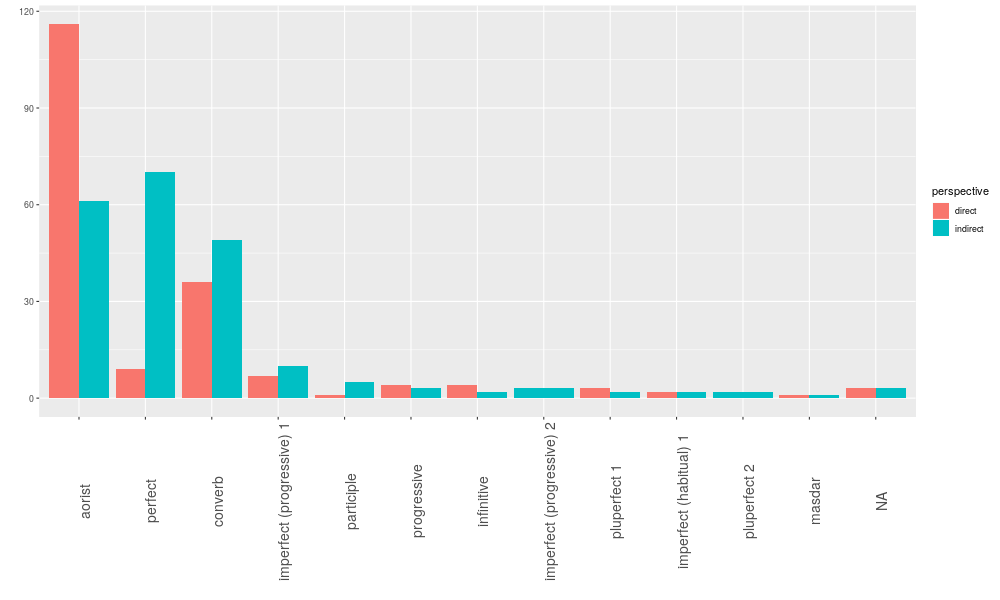
\includegraphics[scale=0.35]{images/andinarr.png}}
\end{figure}

По сравнению с контекстами прямого доступа, употребление Перфекта более приемлемо в незасвидетельствованном контексте. Однако употребление Аориста допустимо и в том случае, если говорящий сам не видел событий, тогда как Перфект в очевидном контексте встречается только в единичных предложениях. Это ожидаемо, потому что, как уже говорилось выше, Перфект в своем неэвиденциальном употреблении не может составлять главную форму в нарративной цепочке. Несмотря на явную количественную корреляцию между формой и перспективой засвидетельствованности, ни один из носителей во время дополнительного обсуждения не называл параметр засвидетельствованности в качестве причины выбора той или иной формы, вне зависимости от диалекта. 
\par По поводу рисунка \ref{fig:nartest} еще стоит отметить, что аналитические формы Аористной серии, представлены в обеих перспективах, тогда как формы Перфектной серии встречаются только в незасвидетельствованных нарративах. Известно, что формы Перфектной серии в своем употреблении более ограничены чем собственно Перфект, потому что для них не характерна такая полисемия, которая ассоциируется с Перфектом. Формы Аористной серии при этом нейтральны, подобно собственно Аористу. Рисунок показывает достаточно убедительное соответствие между перспективой засвидетельствованности и употреблением глагольных форм. Поэтому особенно интересны те случаи, где предположение о перспективе свидетельства как предиктор не оправдалось. Мы рассмотрим структуру конкретных рассказов и случаи отступления от ожидаемых нарративных стратегий. Для этого мы сначала отфильтровали все нефинитные формы, потому что они не относятся к главной линии нарратива. В таблицах \ref{tab:andinardirect} и \ref{tab:andinarindirect} ниже каждому носителю (обозначенному сокращением в верхней строчке) соответствуют два столбца. В левом столбце указана употребляемая форма (pst --- Аорист; pf Перфект; x --- другое), а в правом столбце --- функция предложения, к которому форма/клауза относится (0 --- первое предложение нарратива;  1 --- главная линия).

\begin{table}[H]
\tiny
\caption{Структура рассказов о засвидетельствованных событиях на андийских диалектах}
\label{tab:andinardirect}
\vspace{0.2cm}
\begin{center}
\begin{tabular}{llllllllllllllllllllllllll}
\multicolumn{2}{c}{A}         & \multicolumn{2}{c}{AAJu}                                & \multicolumn{2}{c}{ABE}                                 & \multicolumn{2}{c}{AMKh}                                & \multicolumn{2}{c}{GRG}                                 & \multicolumn{2}{c}{GRSh}                                & \multicolumn{2}{c}{Kh}                                  & \multicolumn{2}{c}{KhMM}                                & \multicolumn{2}{c}{M} & \multicolumn{2}{c}{MKG} & \multicolumn{2}{c}{MShM} & \multicolumn{2}{c}{NNA} & \multicolumn{2}{c}{Z}                                   \\ \hline
\rowcolor[HTML]{C0C0C0} 
x                         & 0 & x                           & 0                         & x                           & 0                         & \cellcolor[HTML]{9AFF99}pst & 0                         & x                           & 0                         & \cellcolor[HTML]{9AFF99}pst & 0                         & \cellcolor[HTML]{9AFF99}pst & 0                         & \cellcolor[HTML]{9AFF99}pst & 0                         & x          & 0        & x           & 0         & x            & 0         & x           & 0         & \cellcolor[HTML]{9AFF99}pst & 0                         \\
\rowcolor[HTML]{9AFF99} 
\cellcolor[HTML]{C0C0C0}x & 1 & pst                         & 1                         & pst                         & 1                         & pst                         & \cellcolor[HTML]{C0C0C0}0 & \cellcolor[HTML]{C0C0C0}x   & 1                         & pst                         & \cellcolor[HTML]{C0C0C0}0 & pst                         & 1                         & \cellcolor[HTML]{C0C0C0}x   & \cellcolor[HTML]{C0C0C0}0 & pst        & 1        & pst         & 1         & pst          & 1         & pst         & 1         & pst                         & 1                         \\
\rowcolor[HTML]{9AFF99} 
pst                       & 1 & \cellcolor[HTML]{C0C0C0}x   & 1                         & pst                         & 1                         & pst                         & 1                         & pst                         & 1                         & \cellcolor[HTML]{C0C0C0}x   & 1                         & \cellcolor[HTML]{C0C0C0}x   & 1                         & pst                         & 1                         & pst        & 1        & pst         & 1         & pst          & 1         & pst         & 1         & pst                         & 1                         \\
\rowcolor[HTML]{9AFF99} 
pst                       & 1 & pst                         & 1                         & pst                         & 1                         & pst                         & 1                         & pst                         & 1                         & \cellcolor[HTML]{C0C0C0}x   & 1                         & pst                         & 1                         & \cellcolor[HTML]{C0C0C0}x   & 1                         & pst        & 1        & pst         & 1         & pst          & 1         & pst         & 1         & pst                         & 1                         \\
\rowcolor[HTML]{9AFF99} 
pst                       & 1 & pst                         & 1                         & pst                         & 1                         & pst                         & 1                         & pst                         & 1                         & pst                         & 1                         & pst                         & 1                         & pst                         & 1                         & pst        & 1        & pst         & 1         & pst          & 1         & pst         & 1         & pst                         & 1                         \\
\rowcolor[HTML]{9AFF99} 
pst                       & 1 & pst                         & 1                         & pst                         & 1                         & pst                         & 1                         & \cellcolor[HTML]{C0C0C0}x   & 1                         & pst                         & 1                         & pst                         & 1                         & pst                         & 1                         & pst        & 1        & pst         & 1         & pst          & 1         & pst         & 1         & pst                         & 1                         \\
\rowcolor[HTML]{9AFF99} 
pst                       & 1 & pst                         & 1                         & pst                         & 1                         & pst                         & 1                         & pst                         & 1                         & pst                         & 1                         & \cellcolor[HTML]{C0C0C0}    & 1                         & \cellcolor[HTML]{FFCCC9}pf  & 1                         & pst        & 1        & pst         & 1         & pst          & 1         & pst         & 1         & \cellcolor[HTML]{FFCCC9}pf  & 1                         \\
\rowcolor[HTML]{9AFF99} 
pst                       & 1 & pst                         & 1                         & pst                         & 1                         & pst                         & 1                         & pst                         & 1                         & pst                         & 1                         & pf                          & 1                         & pst                         & 1                         & pst        & 1        & pst         & 1         & pst          & 1         & pst         & 1         & \cellcolor[HTML]{FFCCC9}pf  & 1                         \\
\rowcolor[HTML]{9AFF99} 
pst                       & 1 & pst                         & 1                         & pst                         & 1                         & pst                         & 1                         & pst                         & 1                         & pst                         & 1                         & pst                         & 1                         & pst                         & 1                         & pst        & 1        & pst         & 1         & pst          & 1         & pst         & 1         & \cellcolor[HTML]{FFCCC9}pf  & 1                         \\
\rowcolor[HTML]{9AFF99} 
pst                       & 1 & pst                         & 1                         & pst                         & 1                         & pst                         & 1                         & pst                         & 1                         & pf                          & 1                         & pst                         & 1                         & \cellcolor[HTML]{FFCCC9}pf  & 1                         & pst        & 1        & pst         & 1         & pst          & 1         & pst         & 1         & \cellcolor[HTML]{FFCCC9}pf  & 1                         \\
                          &   & \cellcolor[HTML]{9AFF99}pst & \cellcolor[HTML]{9AFF99}1 & \cellcolor[HTML]{9AFF99}pst & \cellcolor[HTML]{9AFF99}1 & \cellcolor[HTML]{9AFF99}pst & \cellcolor[HTML]{9AFF99}1 & \cellcolor[HTML]{9AFF99}pst & \cellcolor[HTML]{9AFF99}1 & \cellcolor[HTML]{FFCCC9}pf  & \cellcolor[HTML]{9AFF99}1 & \cellcolor[HTML]{9AFF99}pst & \cellcolor[HTML]{9AFF99}1 & \cellcolor[HTML]{9AFF99}pst & \cellcolor[HTML]{9AFF99}1 &            &          &             &           &              &           &             &           & \cellcolor[HTML]{9AFF99}pst & \cellcolor[HTML]{9AFF99}1 \\
                          &   &                             &                           &                             &                           & \cellcolor[HTML]{9AFF99}pst & \cellcolor[HTML]{9AFF99}1 &                             &                           & \cellcolor[HTML]{9AFF99}pst & \cellcolor[HTML]{9AFF99}1 &                             &                           & \cellcolor[HTML]{9AFF99}pst & \cellcolor[HTML]{9AFF99}1 &            &          &             &           &              &           &             &           &                             &                           \\
                          &   &                             &                           &                             &                           & \cellcolor[HTML]{9AFF99}pst & \cellcolor[HTML]{9AFF99}1 &                             &                           &                             &                           &                             &                           &                             &                           &            &          &             &           &              &           &             &           &                             &                          
\end{tabular}
\end{center}
\end{table}

Первое предложение выделяется потому, что в нем задана рамка для рассказа. Тем самым оно не включено в основную линию, и употребление форм в этом контексте может отличаться от остального нарратива. Зеленым цветом раскрашены клаузы главной линии в правом столбце и ожидаемая форма в левом столбце. В контексте прямой засвидетельствованности, например, мы ожидаем преимущественно Аорист, поэтому Аористы раскрашены зеленым. Встреченные Перфекты (т.е. неожиданные формы) закрашены красным цветом. В таблице \ref{tab:andinarindirect}, наоборот, Перфекты раскрашены зеленым, а Аористы красным цветом, поскольку мы предполагаем, что в незасвидетельствованных нарративах носители предпочитают Перфект. Серым цветом выделяются клаузы первого предложения, а также все нерелевантные для нас формы (т.е. формы все формы кроме Аориста и Перфекта, например, Плюсквамперфект, Имперфект, Проргрессив, и т.д.)

\begin{table}[H]
\tiny
\caption{Структура рассказов о \textit{незасвидетельствованных} событиях на андийских диалектах}
\label{tab:andinarindirect}
\vspace{0.2cm}
\begin{center}
\begin{tabular}{llllllllllllllllllllllllll}
\multicolumn{2}{c}{A}                                   & \multicolumn{2}{c}{AAJu}                                & \multicolumn{2}{c}{ABE}                                 & \multicolumn{2}{c}{AMKh}                                & \multicolumn{2}{c}{GRG}                                 & \multicolumn{2}{c}{GRSh}                                & \multicolumn{2}{c}{Kh}                                  & \multicolumn{2}{c}{KhMM}                               & \multicolumn{2}{c}{M}                                   & \multicolumn{2}{c}{MKG}                                 & \multicolumn{2}{c}{MShM}                                & \multicolumn{2}{c}{NNA}                                 & \multicolumn{2}{c}{Z}                                   \\ \hline
\rowcolor[HTML]{C0C0C0} 
x                           & 0                         & x                           & 0                         & \cellcolor[HTML]{FFCCC9}pst & 0                         & \cellcolor[HTML]{FFCCC9}pst & 0                         & \cellcolor[HTML]{FFCCC9}pst & 0                         & \cellcolor[HTML]{FFCCC9}pst & 0                         & \cellcolor[HTML]{FFCCC9}pst & 0                         & x                          & 0                         & x                           & 0                         & \cellcolor[HTML]{FFCCC9}pst & 0                         & \cellcolor[HTML]{FFCCC9}pst & 0                         & x                           & 0                         & \cellcolor[HTML]{FFCCC9}pst & 0                         \\
\rowcolor[HTML]{C0C0C0} 
x                           & 0                         & x                           & 0                         & x                           & 0                         & \cellcolor[HTML]{FFCCC9}pst & 0                         & x                           & 0                         & \cellcolor[HTML]{FFCCC9}pst & 0                         & \cellcolor[HTML]{9AFF99}pf  & 0                         & x                          & 0                         & \cellcolor[HTML]{FFCCC9}pst & \cellcolor[HTML]{9AFF99}1 & x                           & 0                         & x                           & 0                         & x                           & 0                         & \cellcolor[HTML]{9AFF99}pf  & \cellcolor[HTML]{9AFF99}1 \\
\rowcolor[HTML]{9AFF99} 
\cellcolor[HTML]{C0C0C0}x   & 1                         & \cellcolor[HTML]{FFCCC9}pst & 1                         & \cellcolor[HTML]{C0C0C0}x   & 1                         & \cellcolor[HTML]{FFCCC9}pst & \cellcolor[HTML]{C0C0C0}0 & \cellcolor[HTML]{C0C0C0}x   & \cellcolor[HTML]{C0C0C0}0 & \cellcolor[HTML]{FFCCC9}pst & \cellcolor[HTML]{C0C0C0}0 & pf                          & \cellcolor[HTML]{C0C0C0}0 & pf                         & 1                         & pf                          & 1                         & \cellcolor[HTML]{FFCCC9}pst & 1                         & \cellcolor[HTML]{FFCCC9}pst & 1                         & \cellcolor[HTML]{FFCCC9}pst & 1                         & pf                          & 1                         \\
\rowcolor[HTML]{9AFF99} 
\cellcolor[HTML]{FFCCC9}pst & 1                         & pf                          & 1                         & \cellcolor[HTML]{FFCCC9}pst & 1                         & \cellcolor[HTML]{FFCCC9}pst & 1                         & \cellcolor[HTML]{FFCCC9}pst & 1                         & \cellcolor[HTML]{C0C0C0}x   & 1                         & pf                          & \cellcolor[HTML]{C0C0C0}0 & \cellcolor[HTML]{C0C0C0}x  & 1                         & pf                          & 1                         & pf                          & 1                         & \cellcolor[HTML]{FFCCC9}pst & 1                         & \cellcolor[HTML]{FFCCC9}pst & 1                         & pf                          & 1                         \\
\rowcolor[HTML]{9AFF99} 
\cellcolor[HTML]{FFCCC9}pst & 1                         & pf                          & 1                         & \cellcolor[HTML]{FFCCC9}pst & 1                         & pf                          & 1                         & \cellcolor[HTML]{C0C0C0}x   & 1                         & \cellcolor[HTML]{C0C0C0}x   & 1                         & \cellcolor[HTML]{C0C0C0}x   & 1                         & pf                         & 1                         & pf                          & 1                         & \cellcolor[HTML]{FFCCC9}pst & 1                         & \cellcolor[HTML]{FFCCC9}pst & 1                         & pf                          & 1                         & pf                          & 1                         \\
\rowcolor[HTML]{9AFF99} 
\cellcolor[HTML]{FFCCC9}pst & 1                         & \cellcolor[HTML]{FFCCC9}pst & 1                         & \cellcolor[HTML]{FFCCC9}pst & 1                         & pf                          & 1                         & \cellcolor[HTML]{FFCCC9}pst & 1                         & pf                          & 1                         & \cellcolor[HTML]{C0C0C0}x   & 1                         & pf                         & 1                         & pf                          & 1                         & \cellcolor[HTML]{FFCCC9}pst & 1                         & \cellcolor[HTML]{FFCCC9}pst & 1                         & \cellcolor[HTML]{FFCCC9}pst & 1                         & \cellcolor[HTML]{FFCCC9}pst & 1                         \\
\rowcolor[HTML]{9AFF99} 
\cellcolor[HTML]{FFCCC9}pst & 1                         & pf                          & 1                         & \cellcolor[HTML]{FFCCC9}pst & 1                         & pf                          & 1                         & \cellcolor[HTML]{FFCCC9}pst & 1                         & pf                          & 1                         & pf                          & 1                         & pf                         & 1                         & pf                          & 1                         & \cellcolor[HTML]{FFCCC9}pst & 1                         & \cellcolor[HTML]{FFCCC9}pst & 1                         & pf                          & 1                         & pf                          & 1                         \\
\rowcolor[HTML]{9AFF99} 
\cellcolor[HTML]{FFCCC9}pst & 1                         & pf                          & 1                         & \cellcolor[HTML]{FFCCC9}pst & 1                         & pf                          & 1                         & \cellcolor[HTML]{FFCCC9}pst & 1                         & pf                          & 1                         & pf                          & 1                         & pf                         & 1                         & pf                          & 1                         & pf                          & 1                         & \cellcolor[HTML]{FFCCC9}pst & 1                         & pf                          & 1                         & pf                          & 1                         \\
\rowcolor[HTML]{9AFF99} 
pf                          & 1                         & pf                          & 1                         & \cellcolor[HTML]{FFCCC9}pst & 1                         & pf                          & 1                         & \cellcolor[HTML]{FFCCC9}pst & 1                         & pf                          & 1                         & pf                          & 1                         & pf                         & 1                         & pf                          & 1                         & pf                          & 1                         & \cellcolor[HTML]{FFCCC9}pst & 1                         & pf                          & 1                         & pf                          & 1                         \\
\rowcolor[HTML]{9AFF99} 
\cellcolor[HTML]{FFCCC9}pst & 1                         & \cellcolor[HTML]{FFCCC9}pst & 1                         & \cellcolor[HTML]{FFCCC9}pst & 1                         & pf                          & 1                         & pf                          & 1                         & pf                          & 1                         & pf                          & 1                         & pf                         & 1                         & pf                          & 1                         & \cellcolor[HTML]{FFCCC9}pst & 1                         & \cellcolor[HTML]{FFCCC9}pst & 1                         & pf                          & 1                         & \cellcolor[HTML]{FFCCC9}pst & 1                         \\
\cellcolor[HTML]{9AFF99}pf  & \cellcolor[HTML]{9AFF99}1 & \cellcolor[HTML]{9AFF99}pf  & \cellcolor[HTML]{9AFF99}1 & \cellcolor[HTML]{FFCCC9}pst & \cellcolor[HTML]{9AFF99}1 & \cellcolor[HTML]{9AFF99}pf  & \cellcolor[HTML]{9AFF99}1 & \cellcolor[HTML]{FFCCC9}pst & \cellcolor[HTML]{9AFF99}1 & \cellcolor[HTML]{9AFF99}pf  & \cellcolor[HTML]{9AFF99}1 & \cellcolor[HTML]{9AFF99}pf  & \cellcolor[HTML]{9AFF99}1 & \cellcolor[HTML]{9AFF99}pf & \cellcolor[HTML]{9AFF99}1 & \cellcolor[HTML]{9AFF99}pf  & \cellcolor[HTML]{9AFF99}1 & \cellcolor[HTML]{FFCCC9}pst & \cellcolor[HTML]{9AFF99}1 & \cellcolor[HTML]{FFCCC9}pst & \cellcolor[HTML]{9AFF99}1 & \cellcolor[HTML]{9AFF99}pf  & \cellcolor[HTML]{9AFF99}1 &                             &                           \\
                            &                           &                             &                           &                             &                           & \cellcolor[HTML]{9AFF99}pf  & \cellcolor[HTML]{9AFF99}1 & \cellcolor[HTML]{FFCCC9}pst & \cellcolor[HTML]{9AFF99}1 & \cellcolor[HTML]{9AFF99}pf  & \cellcolor[HTML]{9AFF99}1 & \cellcolor[HTML]{9AFF99}pf  & \cellcolor[HTML]{9AFF99}1 & \cellcolor[HTML]{9AFF99}pf & \cellcolor[HTML]{9AFF99}1 &                             &                           & \cellcolor[HTML]{C0C0C0}x   & \cellcolor[HTML]{9AFF99}1 &                             &                           &                             &                           &                             &                           \\
                            &                           &                             &                           &                             &                           &                             &                           & \cellcolor[HTML]{FFCCC9}pst & \cellcolor[HTML]{9AFF99}1 & \cellcolor[HTML]{FFCCC9}pst & \cellcolor[HTML]{9AFF99}1 & \cellcolor[HTML]{9AFF99}pf  & \cellcolor[HTML]{9AFF99}1 & \cellcolor[HTML]{9AFF99}pf & \cellcolor[HTML]{9AFF99}1 &                             &                           & \cellcolor[HTML]{FFCCC9}pst & \cellcolor[HTML]{9AFF99}1 &                             &                           &                             &                           &                             &                          
\end{tabular}
\end{center}
\end{table}

Опираясь на таблицу \ref{tab:andinarindirect}, можно сказать, что из 13 носителей 8 использовали стратегию с Перфектом для заглазного нарратива, т.е., основная линия рассказа оформлена цепочкой Перфектов. Два носителя (AMKhA и NNA) начали рассказ в Аористе, после чего переключились на Перфект. Интересно отметить, что к Аористам в версии NNA, единственного представителя мунинского диалекта в нашей выборке, присоединяется Репортативная Частица (\textit{godi}), тогда как к Перфектам в той же цепочке она не добавляется. У трёх носителей (AAJu, MKG и Z) Перфекты с Аористами чередуются. Таблицы \ref{tab:andinarindirect} и \ref{tab:andinardirect} подтверждают, что Перфектная стратегия допускается только в незасвидетельствованном контексте. Сравнение с таблицей \ref{tab:andinarindirect} при этом позволяет утверждать, что преобладание Аориста в засвидетельствованном контексте связано скорее с недопустимостью употребления в этом контексте Перфекта и ничего не говорит о том, насколько грамматикализованно значение очевидности. Отсутствие Перфектной стратегии в косвенных нарративах у нескольких носителей можно объяснить тем, что Аорист нейтрален в плане эвиденциальности, так что выбор формы определяется нарративными предпочтениями говорящего. При этом на носителей могла влиять формулировка первого предложения. Поскольку в нем дословно указан источник информации (<<Мне рассказывали, что..>>), это можно воспринимать как своего рода нарративное обрамление, после чего дальнейшие указания на источник информации в принципе не нужны. Считающаяся типичной стратегия обрамления, при которой говорящий начинает рассказ в Перфекте, после чего переключается на Аорист в качестве общего прошедшего, в наших элицитациях не представлена.
\par Среди тех носителей, которые выбрали Аористную стратегию в косвенном нарративе, были 4 из 5 носителей рикванинского диалекта. Это любопытный результат, поскольку данные анкетирования, обсуждаемые в разделе \ref{sec:elicitation}, казалось бы, указывали на то, что в рикванинском Перфект как показатель косвенной засвидетельствованности более грамматикализован, чем в зиловском диалекте. В то же время, 5 из 6 носителей зиловского диалекта употребляют в косвенном нарративе Перфектную стратегию. Вопрос о том, насколько это соответствие характерно для каждого диалекта в целом или же лишь для определенных носителей, требует дальнейшего изучения. Из двух носителей, которые не использовали ни одного Перфекта в косвенном контексте, один использовал репортативную частицу. Репортативная частица также употребляется носителем Kh на одном из главных предикатов первого предложения перевода, причем предикат этот стоит в форме Перфекта. Дальше рассказ продолжается полностью в Перфекте, ср. первое предложение в (\ref{ex:ziloberries1}) и второе предложение в (\ref{ex:ziloberries2}), с Плюсквамперфектом серии Перфекта.

\lb{ex:ziloberries1}{\gll di-qi \textbf{bosːon} di-j ila reš-ƛi j-iʔon-nij ʁurʁi r-ak’arun-nij \textbf{j-iʔo-j=ʁodi}\\
{\First}{\Sg}-{\Ad} tell.{\Aor} {\First}{\Sg}-{\F}[{\Gen}] mother forest-{\Inter} {\F}-go-{\Pf} blackcurrant {\Inantwo}-gather-{\Pf} {\F}-go-{\Pf}={\Rep}\\
\trans `Мне \textbf{рассказывали}, что моя мать пошла в лес, \textbf{пошла} собирать смородину.' \\ \footnotesize{[полевая работа 2017-го года] \hfill андийский: зиловский}}

\vfill
\pagebreak

\lb{ex:ziloberries2}{\gll χʷant’ulo=lo \textbf{j-ik’o-j} \textbf{r-ak’arun-nij}\\
whole\_day={\Add} {\F}-be-{\Pf} {\Inantwo}-gather-{\Pf}\\
\trans `Она собирала весь день.' \\ \footnotesize{[полевая работа 2017-го года] \hfill андийский: зиловский}}

Стоит отметить, что никто из носителей не использовал Репортатив на каждом главном предикате, хотя такая стратегия представлена в материале, записанном Я.Г. Сулеймановым на рикванинском диалекте, см. сказку про лису и перепёлку в \citep[423]{sulejmanov1957}. Отмеченные переходы от одной формы к другой в пределах нарратива связаны с информационной структурой: переход от Аориста к Перфекту выдвигает действие на передний план и поэтому встречается преимущественно в предложениях 7, 8, и 9 (вне зависимости от эвиденциальной перспективы), когда главный персонаж нечаянно наступает на змею (7), после чего змея кусает его/ее (8), а он(а) бросает в змею камень (9). При этом решение о том, на каком именно из этих событий делать акцент, варьируется у разных носителей. Переход от Перфекта к Аористу, наоборот, обозначает <<логическое следствие>> из предыдущего действия. Например, переход от Перфекта к Аористу в последнем предложении (`змея умерла') носитель объяснил тем, что это логическое следствие того, что змею ударили камнем в предыдущем предложении, хотя в этой ситуации можно продолжать нарратив и в Перфекте. Решения о переключениях очень индивидуальны, и, в принципе, как показывают переводы нескольких носителей, при построении нарратива можно вовсе обойтись без них. Стоит отметить, что здесь появляется ассиметрия --- переключение из Аориста в Перфект имеет другое значение чем переход от Перфекта в Аорист, тогда как их роль в главной линии аналогична.
\par Результаты эксперимента показывают, что употребление Аориста и Перфекта в андийских диалектах связано с эвиденциальной перспективой, что отражается в количестве Перфектов в нарративах, построенных из разных перспектив (см. рисунок \ref{fig:nartest}). При этом носители не обязательно ощущают эвиденциальную семантику --- из тех носителей, которые применяли перфектоидную стратегию в заглазном контексте, ни один не назвал засвидетельствованность в качестве причины выбора соответствующих форм. Некоторые в обоих контекстах употребляют немаркированный Аорист. Стоит при этом иметь в виду, что данный эксперимент также является элицитацией, соответственно, факторы, обсуждаемые выше в разделе \ref{sec:elicitation}, могли отчасти влиять на выбор форм и искажать картину. Тем не менее, в записанных на андийском языке рассказах, например, в грамматических очерках \citep{dirr1906}, \citep{sulejmanov1957}, \citep{tsertsvadze65}, \citep{salimov2010}, представлены все те же стратегии: перфектоидная стратегия в заглазном контексте, аористная стратегия в очевидном и заглазном контекстах, стратегия с репортативом и нарративы с переключениями между формами. 
%В следующем разделе мы рассмотрим неэлицитированные тексты на двух других языках. Данные из спонтанной речи, естественно, более сложны для анализа, чем простые элицитированные цепочки, которые обсуждались в настоящем разделе. В связи с этим мы сначала обсудим теоретические подходы к дейктическим категориям (включая эвиденциальность) в нарративном режиме, а также параметры, используемые для интерпретации разных функций глагольных форм в этом контексте.

\section{Нарративное употребление как самостоятельный признак} \label{sec:svod}

Данные андийского языка, представленные в предыдущем разделе \ref{sec:andinarr}, вызывают следующий, немаловажный для целей нашего исследования вопрос: возможно ли, что употребление перфектоида в качестве прошедшего заглазного в нарративном контексте является независимым свойством данной категории? Как обсуждалось в разделе \ref{sec:andinarr}, эвиденциальная семантика слабо (или вовсе не) ощущается большинством носителей разных диалектов андийского языка, которых мы опрашивали, в отличие, например, от носителей ингушского языка, которые ярко осознают эти различия \citep[243]{nichols2011}. Среди носителей зиловского диалекта, с которыми мы работали, нет ни одного, кто назвал бы параметр засвидетельствованности в качестве причины выбора той или иной формы. В то же время они последовательно применяют перфектоидную нарративную стратегию для рассказов о незасвидетельствованных событиях не только при элицитации, но и в естественных нарративах.\footnote{Корпус текстов на зиловском диалекте андийского языка пока в процессе обработки.} Для этого противоречия возможно несколько разных объяснений:

\pagebreak

\begin{enumerate}
    \item Эвиденциальная семантика в других контекстах всё же присутствует, но анкетирование оказалось неудачным или было проведено с выборкой носителей, нерепрезентативной для языкового (или диалектного) сообщества в целом.
    \item Эвиденциальная семантика вне нарративного контекста ранее ощущалась более ярко, но утрачивается или уже утрачена, в то время как нарратив оказался устойчивым контекстом из-за его связи с традициями устного творчества.\footnote{А.Ю. Айхенвальд \citep[301]{aikhenvald2004} отмечает, что утрата нарративных традиций может становиться причиной утраты категории эвиденциальности. Возможно в данном случае, наоборот, традиция устной литературы поддерживает сохранение категории.}
    \item Нарративное употребление --- самостоятельный признак, присутствие которого необязательно подразумевает, что форма имеет или когда-либо имела заглазное значение в других дискурсивных или морфосинтаксических контекстах.
\end{enumerate}

Первое объяснение представляется нам маловероятным. Мы опросили больше десяти разных носителей зиловского диалекта, что для исследования такой темы в бесписьменном языке представляется - по сравнению с другими исследованиями - достаточно широкой выборкой.\footnote{Кроме эксперимента с элицитацией рассказов, мы проходили анкеты по разным темам с другими носителями и задавали носителям дополнительные вопросы о контрастах и причинах выбора тех или иных форм.} К тому же, несмотря на то, что у носителей аварского языка и рикванинского диалекта андийского языка также наблюдаются колебания в оценке наличия и роли эвиденциальной семантики, среди них всё же находились и такие, кто выделял фактор засвидетельствованности (впрочем, для этих языков мы опросили намного меньше носителей --- три носителя аварского языка, исключая тех, кого мы попросили лишь интерпретировать разницу между двумя короткими нарративами, как обсуждалось в разделе \ref{sec:elicitation}, и пять носителей рикванинского диалекта). Данные опроса нельзя считать доказательством того, что эвиденциальный компонент значения в интуиции носителей зиловского полностью отсутствует; однако, как кажется, их можно считать указанием на то, что этот компонент присутствует менее ярко по сравнению с другими диалектами и языками. 
\par Второе возможное объяснение кажется правдоподобным, поскольку (народная) литература часто служит контекстом сохранения архаичных языковых черт. Однако в отсутствие эвиденциальных прочтений вне нарративного контекста сложно счесть именно это объяснение как более вероятным по сравнению с третьим. Именно третье объяснение представляет наиболее серьезную проблему для настоящего исследования. Мы предположили, что нарративное употребление --- стабильный, однозначный признак степени грамматикализованности заглазного значения, ср. \ref{sec:pftyp}. Если же данную функцию можно считать независимым признаком, то ее нельзя связать со степенью грамматикализованности категории эвиденциальности. Правда, кажется маловероятным, чтобы употребление перфектоида как заглазного прошедшего может появиться в  (нахско-дагестанском) языке как бы из ничего, вообще без посредства постепенной эволюции из инферентива, как было описано в разделе \ref{sec:pftyp}. Тем не менее, если учитывать контакт с другими языками, в которых заглазность грамматикализована и перфектоид употребляется в заглазных нарративах, нельзя исключить сценарий, в котором нарративное употребление перфектоида заимствуется как стилистический прием, характерный для определенного фольклорного жанра (или совокупности жанров). Поэтому мы решили провести дополнительный анализ нарративных стратегий, используемых в фольклорных текстах на разных дагестанских языках.


\begin{table}[ht]
\caption{Нарративные стратегии в фольклорных текстах}
\centering
\label{tab:svod}
\vspace{0.5cm}
\begin{tabular}{lll}
\multicolumn{1}{c}{Язык}        & \multicolumn{1}{c}{Том Свода}                      & \multicolumn{1}{c}{Стратегия} \\ \hline
\multicolumn{1}{l|}{кумыкский}  & \multicolumn{1}{l|}{1. Сказки о животных}    & перфектоид                    \\
\multicolumn{1}{l|}{}           & \multicolumn{1}{l|}{2. Волшебные сказки}     & перфектоид                    \\
\multicolumn{1}{l|}{}           & \multicolumn{1}{l|}{3. Бытовые сказки}       & перфектоид                    \\
\multicolumn{1}{l|}{}           & \multicolumn{1}{l|}{4. Мифологическая проза} & перфектоид                    \\ \hline
\multicolumn{1}{l|}{аварский}   & \multicolumn{1}{l|}{1. Сказки о животных}    & перфектоид / репортатив       \\
\multicolumn{1}{l|}{}           & \multicolumn{1}{l|}{2. Волшебные сказки}     & репортатив                    \\
\multicolumn{1}{l|}{}           & \multicolumn{1}{l|}{3. Бытовые сказки}       & репортатив                    \\
\multicolumn{1}{l|}{}           & \multicolumn{1}{l|}{4. Мифологическая проза} & перфектоид                    \\ \hline
\multicolumn{1}{l|}{рутульский} & \multicolumn{1}{l|}{1. Сказки о животных}    & презенс / аорист            \\
\multicolumn{1}{l|}{}           & \multicolumn{1}{l|}{2. Волшебные сказки}     & презенс / аорист            \\
\multicolumn{1}{l|}{}           & \multicolumn{1}{l|}{3. Бытовые сказки}       & презенс / аорист            \\
\multicolumn{1}{l|}{}           & \multicolumn{1}{l|}{4. Мифологическая проза} & презенс / аорист            \\ \hline
\multicolumn{1}{l|}{лезгинский} & \multicolumn{1}{l|}{1. Сказки о животных}    & аорист                        \\
\multicolumn{1}{l|}{}           & \multicolumn{1}{l|}{2. Волшебные сказки}     & аорист                        \\
\multicolumn{1}{l|}{}           & \multicolumn{1}{l|}{3. Бытовые сказки}       & аорист                        \\
\multicolumn{1}{l|}{}           & \multicolumn{1}{l|}{4. Мифологическая проза} & аорист                       
\end{tabular}
\end{table}

\par В разделе \ref{sec:maps} было показано, что, согласно существующей литературе, заглазное значение перфектоида отсутствует в нескольких языках Южного Дагестана (в рутульском, табасаранском, лезгинском, хиналугском, будухском и удинском языках), хотя для лезгинского и хиналугского языков имеются ограниченные сведения о наличии по крайней мере инферентивной интерпретации этой формы, ср. обсуждение в разделе \ref{sec:maps}. %это тот раздел?
Лезгинский, рутульский и в меньшей степени табасаранский языки представлены в \textit{Своде памятников фольклора народов Дагестана}.\footnote{Из 20 планированных томов данной антологии, до 2019-го года вышли первые шесть: \textit{1. Сказки о животных} \citep{svod1}, \textit{2. Волшебные сказки} \citep{svod2}, \textit{3. Бытовые сказки} \citep{svod3}, \textit{4. Мифологическая проза} \citep{svod4}, \textit{5. Героический и героико-исторический эпос} \citep{svod5}, \textit{6. Обрядовая поэзия} \citep{svod6}.} В <<Своде>> представлены памятники из архива фольклорных текстов --- оригинальные тексты на языках Дагестана с переводом на русский язык. Кроме вышеперечисленных языков, представлены также тексты на аварском и кумыкском языках и (немного меньше) на агульском и ногайском языках, а также, в пятом томе \citep{svod5}, один текст на азербайджанском языке. Мы случайным образом выбрали по четыре текста из четырех томов: один на аварском языке, один на кумыкском, один на рутульском и один на лезгинском языке, и сравнили стратегии оформления главной линии рассказа: результаты представлены в таблице \ref{tab:svod}.\footnote{Полную таблицу с указанием на конкретные тексты, которые мы расcмотрели, можно найти по ссылке: \url{https://github.com/sverhees/dissertation_evidentiality}.} Мы выбрали именно эти четыре тома в связи с тем, что поэзия и эпос отличаются от сказок в плане стиля повествования, а эпические сказания представлены к тому же не для всех языков --- в пятом томе Свода, например, отсутствует рутульский материал. Как показывает таблица \ref{tab:svod}, в кумыкском все четыре текста оформляются перфектоидной стратегией (т.е., формой с суффиксом \textit{-ʁan} или \textit{-gan}, как в тексте <<Бусы Вайкут-майкут>> из четвертого тома, на кайтагском диалекте). В аварском языке перфектоидная стратегия конкурирует с репортативной, при которой репортатив \textit{ila} оформляет все главные предикаты. Рутульские рассказчики сочетают формы основного прошедшего (аорист, состоящий из перфективного конверба на \textit{-ɨr} и морфологизированной связки \textit{i}) с настоящим временем. В лезгинских текстах преобладает аорист с суффиксом \textit{-na}, который идентичен конвербу. В рутульских и лезгинских текстах перфектоиды встречаются только в единичных случаях при передаче чужой речи. Эти данные не представляют полную картину употребления форм в главной линии фольклорных рассказов на рассматриваемых нами языках, но в целом они соответствуют обобщениям, вытекающим из материала второй главы. Таким образом, можно сделать вывод, что употребление перфектоида в нарративах о незасвидетельствованных или вымышленных событиях скорее всего не появляется независимо, так что наличие таких употреблений можно считать для перфектоидов признаком сильной грамматикализованности эвиденциальной семантики, а отсутствие эвиденциальности в интуиции носителей тех или иных языков указывает скорее на утрату категории в ненарративном дискурсе, чем на ее исходное отсутствие.

\section{Метод анализа нарративных текстов} \label{sec:methodanalysis}

В разделе \ref{sec:cat} мы обсуждали интерпретацию эвиденциальности как дейктической категории на основе ее индексальных свойствах, по аналогии с временным и пространственным дейксисом. Значение таких категорий по умолчанию определяется относительно говорящего и момента речи, его временных и пространственных параметров. Как уже обсуждалось в разделе \ref{sec:cat}, термин <<дейктический>> возможно не является самым уместным. Возможными альтернативами являются - индексальный \citep{hanks2014}, шифтерный \citep{jakobson1957}, эгоцентричный \citep{paducheva2010}\footnote{В работе \citep{paducheva2010} эвиденциальность не обсуждается, поскольку в русском языке нет грамматической эвиденциальности, однако ее анализ модальных и дискурсивных форм можно применить и к эвиденциальным формам.} или clausal grounding в рамках теории когнитивной грамматики \citep{langacker2017}, ср. также \citep{boye2018}. Дейктические подходы опираются на идею о разных воплощениях говорящего в речевых актах. В человеческом языке говорящий играет несколько разных ролей, которые могут совпадать или расходиться. В простом нарративе говорящий может, например, рассказывать про свой личный опыт, про события, в которых он сам играл определенную роль, или же передавать то, что он лично наблюдал. Подходы Х. Бергквиста и П. Коккелмана различают три разные роли говорящего: автор, озвучиватель, поручатель \citep{bergqvist2018}, \citep{kockelman2004}. Поскольку автор составляет высказывание, он главным образом отвечает за перспективизацию. Например, при рассказе о действиях в прошлом автор может выбирать разные временные формы для главной линии своего нарратива (прошедшее, настоящее в качестве praesens historicum, и т.д.), которые имеют определенный дискурсивный эффект. 
\par При оформлении перспективы порождается некий  <<наблюдатель>>, отличный от говорящего, см. раздел \ref{sec:cat}. Образно говоря, наблюдатель является воплощением референциальной гибкости говорящего --- он может путешествовать во времени и в пространстве, помещая себя в ситуациях, в которых он на самом деле не участвовал и при которых не присутствовал. В настоящей работе мы разбиваем высказывание на четыре компонента и выделяем, соответственно, четыре роли. Во-первых, имеется исходное событие, которое происходит в определенном месте, в определенный момент времени и с определенными участниками. Автор дейктически кодирует событие, располагая его во времени и в пространстве и уточняя свое отношение к нему с помощью категорий лица и эвиденциальности. В тех случаях, когда автор полностью совпадает с озвучивателем, время, пространство и другие дейктические измерения определяются относительно момента речи, то есть говорящего.

\lb{ex:botguns}{\gll hu-b zamana-di b-uk’-ič’a ida jaraʁ \textbf{hena} \textbf{iƛi-b=cːu-b}\\
{\Dem}-{\N}	time-{\Erg}	{\N}-be-{\Neg}.{\Cvb} {\Cop} weapons now {\First}{\Pl}.{\Incl}-{\N}={\Comp}-{\N}[{\Gen}]\\
\trans `В то время не было оружия \textbf{как у нас сейчас}.' \footnotesize{\\
\citep{gudava1962} \hfill ботлихский язык}}

В примере (\ref{ex:botguns}), говорящий рассказывает про историю села Ботлих. Озувчиватель в этом случае совпадает с автором, и говорящий рассказывает с собственной точки зрения о событиях которые произошли давно и которые он сам не засвидетельствовал (что объясняет употребление Перфекта \textit{b-uk’-ič’a ida} `было’). При этом он указывает на настоящий момент через комментарий о наличии оружия, включая адресата в дейктический центр использованием инклюзивного местоимения. Особенность роли автора заключается в том, что он способен на перемещение и рекурсию, осуществляемые через фигуру наблюдателя, и может увеличивать или сокращать дистанцию между событием и моментом речи. Таким образом, автор может вводить других авторов и последовательно принимать их перспективу. Озвучиватель в свою очередь может передать перспективу другого автора. В текстах на рикванинском диалекте андийского, записанных Я.Г. Сулеймановым, есть один короткий рассказ о том, как дедушка говорящего ходил продавать андийские бурки, чтобы потом можно было купить ткань. В первом предложении говорящий говорит, что эту историю ему рассказывал дед, после чего он сразу переключается на перспективу первого лица на протяжение всего рассказа, как бы передавая историю от имени своего деда. Интересно заметить, что в переводе к тексту используется местоимение третьего лица.

\lb{ex:burki}{\gll b-aχoɬi murtil=lojd \textbf{išːil} w-ol’on tuken-ni\\
{\Inanone}-sell.{\Aor}({\Cvb}) burka={\Sbr} {\First}{\Sg}.{\Excl} {\M}-{\Pl}.go.{\Aor} store-{\In}.{\Lat}\\
\trans `Продали \textbf{они} бурки и пошли в магазин.'\\
букв. `Продав бурки, мы пошли в магазин.’ \footnotesize{\\ \citep[~421]{sulejmanov1957} \hfill андийский: рикванинский}}

В обычном, утвердительном высказывании поручатель совпадает с автором и озвучивателем. Озвучиватель при этом может передать высказывание, автором которого он не является, и в таком случае он может как ручаться, так и не ручаться за передаваемую информацию. Автор и поручатель могут различаться в том случае, если автор вводит нового автора --- первый автор в таком случае может дистанцироваться от слов нового автора, опровергать их, или наоборот ручаться за них.

\begin{figure}[h]
\centering
\caption{Компоненты высказывания о событии}
\label{fig:roles}
\vspace{0.5cm}

\begin{tabular}{lll}
\textbf{Событие}      & \textbf{} & \textbf{Роль говорящего}                       \\
событие               & →         & участник: участвует в передаваемом событии     \\
событие рассказывания & →         & автор: сочиняет высказывание, кодирует дейксис \\
событие коммитмента   & →         & поручатель: ручается за подлинность информации             \\
момент речи           & →         & озвучиватель: произносит высказывание                       
\end{tabular}
\end{figure}

Х. Бергквист постулировал отдельное событие получения информации (source event), и соответствующую роль для говорящего: восприниматель (cognizer), хотя нам кажется, что такой дополнительный слой --- лишний. Расхождения между событием и событием рассказывания в плане эвиденциальности кодируются автором, и соответственно объясняются разного рода расхождениями между участниками события и автором рассказывания. Поскольку автор дейктически оформляет исходное событие, он отвечает не только за установление связи между этим событием и моментом речи, но и за внутреннюю структуру передаваемого события. Для анализа внутренней структуры ключевым понятием является \textsc{точка отсчета} (point of reference), которое было введено Х. Рейхенбахом для толкования английского Плюсквамперфекта (past perfect), который сочетает семантику прошедшего времени с предшествованием \citep{reichenbach1947}, как в примере (\ref{ex:fred1}): оба события произошли в прошедшем, но отправление Фреда в путь (\textsc{плюсквамперфект}) предшествовало его прибытию (\textsc{простое прошедшее}). Точкой отчета для плюсквамперфекта тем самым является другое событие в контексте, тогда как простое прошедшее определяется относительно момента речи.

\lb{ex:fred1}{Fred arrived at 10. He had set off at 6.\\
\citep[~593]{kampreyle1993}}

В нарративной цепочке плюсквамперфект может передавать последовательные события, которые произошли перед другим событием. В примере (\ref{ex:fred2}) все формы плюсквамперфекта имеют одну и ту же точку отсчета (прибытие Фреда), в то время как по отношению друг к другу они обозначают последовательные (а не предшествующие) события: Фред сначала встал, потом принял душ, и так далее. Эти примеры показывает, что для анализа употребления видо-временных форм в нарративе, помимо самого события и момента речи, важны также точка отсчета (пример (\ref{ex:fred1})) и фигура наблюдателя (пример (\ref{ex:fred2})).

\lb{ex:fred2}{Fred arrived at 10. He had got up at 5; he had taken a long shower, had got dressed and had eaten a leisurely breakfast. He had left the house at 6:30.\\
\citep[~594]{kampreyle1993}}

Для настоящего исследования компонент точки отсчета является релевантным, поскольку формы глагольной парадигмы, о которых идет речь, совмещают разные функции, выбор между которыми осуществляется в контексте, подобно тому, как это происходит с английским плюсквамперфектом. Как было показано в предыдущем разделе, для интерпретации временных форм в рассказах на андийском языке форма, непосредственно предшествующая другой формы в тексте, тоже имеет значение для интерпретации последней. Например, переключение из Аориста в Перфект дает определенный дискурсивный эффект, отсутствующий в цепочке однородных форм.

\subsection{Нарративная цепочка} \label{sec:narseq}

Когда мы используем термин нарратив, мы имеем в виду нарративную цепочку, в которой последовательность событий описывается цепочкой клауз, причем линейный порядок последних отражает порядок последовательности исходных событий во времени. Такие нарративные тексты относительно однородны в плане используемых глагольных форм. При этом нарративный текст имеет такую особенность, что цепочка глагольных форм интерпретируется одинаковым образом, как обозначение последовательности событий. Это касается не только прошедшего общего, но и настоящего, и даже плюсквамперфектов (ср. пример (\ref{ex:fred2}) в разделе \ref{sec:methodanalysis}). Такие примеры объясняются особой ролью наблюдателя в нарративном режиме (по сравнению с речевым режимом) \citep{paducheva2010}. В нарративном режиме, наблюдатель двигается по временной оси параллельно рассказываемым событиям, и цепочка из двух или более одинаковых форм приобретает значение последовательности.
\par Тексты из грамматик, которые были использованы для исследования в разделе \ref{sec:results}, представляют разные жанры, включая как цельные нарративы, так и диалоги. Из каждого текста мы выделили именно нарративные цепочки. Так, например, мы использовали текст о школе, в котором говорящий сначала рассказывает, как организовывали школу и как раньше приезжали русские учителя, которых все очень уважали; и что среди них была одна учительница, которую все особенно полюбили. Рассказывая про эту учительницу, он вспоминает, как однажды она очень сильно заболела и все сельчане ей помогали, но она так и не выздоровела. В итоге ее вывезли на вертолете в больницу в Баку. В наш анализ мы включаем не весь текст, а только этот нарративный эпизод. Также нами не были включены в нарративный текст вводные замечания перед рассказом. Пример (\ref{ex:intro}) представляет переводы первых предложений одного текста на цахурском языке \citep[759--765]{tsakhurgram}. Первые три предложения представляют введение и не относятся к нарративной цепочке, которая начинается только с четвертого предложения.

\lb{ex:intro}{1. Я хочу рассказать историю [=сделать рассказ], которая случилась давным-давно [во время времен бывшую].\\
2. В то время дагестанцы (часто) воевали [=войну делали] с грузинами.\\
3. Эту историю мне рассказал мой дед, а деду — его дед.\\
\textbf{4. Один человек по имени Саид (вместе) со своим другом Исой шел через горы.}}

Вслед за \citep{paducheva2010} мы считаем, что минимальная длина для цепочки составляет две клаузы, с уточнением, что эти клаузы должны быть финитными. В разделе \ref{sec:annotation} подробно описано, как мы размечали разные виды клауз которые встречаются в нарративах.

\vfill
\pagebreak

\section{Выборка языков и данные} \label{sec:sample}

Здесь мы рассматриваем нарративы из текстов на багвалинском языке андийской ветви и на цахурском языке лезгинской ветви. Выбор именно этих языков обоснован, во-первых, наличием (небольших) собраний глоссированных текстов \citep{tsakhurgram}, \citep{bagvalalgram}, и, во-вторых, тем, что эти языки принадлежат разным генеалогическим группам и распространены в географически удаленных друг от друга частях Дагестана, относясь к разным <<зонам влияния>> (ср. раздел \ref{sec:ndlang}). На рисунке \ref{fig:kvanmish} ниже изображены сёла идиомов, которые представлены в наших данных (Кванада для багвалинского и Мишлеш для цахурского) на фоне общего ареала языковых групп. Согласно имеющейся литературе, перфектоиды в этих языках обладают разным статусом. Иногда интерпретация семантики перфектоидов может зависит от автора (см. раздел \ref{sec:pftyp}), но поскольку багвалинским и цахурским занимались одни и те же исследователи, кажется вероятным, что описанные разницы не мотивируются разными теоретическими установками и исследовательскими приемами, и перфектоиды в этих языках действительно чем-то существенно различаются.

\begin{figure}[h]
\centering
\caption{Селения Кванада (багвалинский) и Мишлеш (цахурский) на фоне распределения генеалогических групп языков нахско-дагестанской семьи}
\label{fig:kvanmish}
\vspace{0.5cm}
\fbox{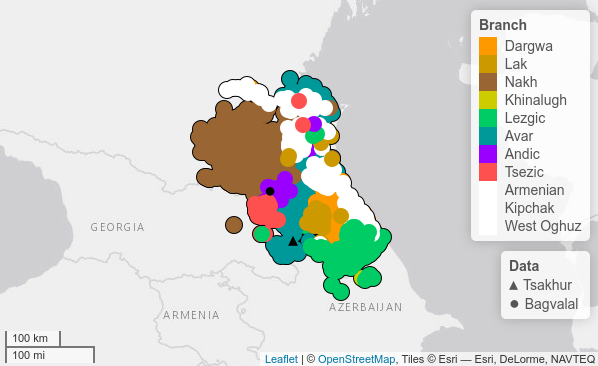
\includegraphics[scale=0.7]{images/kvanmish.png}}
\end{figure}

\subsection{Языки} \label{sec:samplelanguages}

На багвалинском языке говорят около семи тысячи человек в четырёх селениях Цумадинского района и в двух селениях Ахвахского района на северо-западе Дагестана \citep[21]{bagvalalgram}. Носителей цахурского языка от 30 до 50 тысяч \citep[3]{tsakhurgram}, и проживают они в Рутульском районе Дагестана и в граничащих с ним Гахском и Закатальском районах Азербайджана. Как было показано на карте на рисунке \ref{fig:ecvill}, разные языки и ветви нахско-дагестанской семьи в целом географически компактны. В результате среди соседей багвалинского языка мы находим в основном другие андийские языки и аварский язык, а цахурский язык окружён другими лезгинскими языками (лезгинский, рутульский) и азербайджанским.
\par \textbf{Багвалинская система} прошедшего времени типична для аваро-андийских языков. Имеется прошедшее общее (Претерит) и многофункциональный перфектоид (Перфект) со значениями результатива, текущей релевантности, косвенной засвидетельствованности и миративности.\footnote{Впрочем, текущая релевантность присутствует ограниченно, ср. \citep{tatevosov2001}.} Другие формы прошедшего времени образуются вспомогательным глаголом в Претерите, а их заглазные эквиваленты — вспомогательным глаголом в форме Перфекта, см. часть парадигмы в таблице \ref{tab:bagvparad}.

\begin{table}[H]
\caption{Основные формы прошедшего времени глагола \textit{hec’i} ‘подниматься, вставать’ в багвалинском языке, по \citep[394]{maisaktatevosov2001}}
\label{tab:bagvparad}
\vspace{0.2cm}
\begin{center}
\begin{tabular}{lll}
                                            & \begin{tabular}[c]{@{}l@{}}Претерит\\ hec'i\end{tabular} & \begin{tabular}[c]{@{}l@{}}Перфект\\ hec'i-b-o ek'ʷa\end{tabular} \\ \hline
\multicolumn{1}{l|}{Плюсквамперфект}        & hec'i-b-o b-uk'a                                         & hec'i-b-o b-uk'a-b-o ek'ʷa                                        \\
\multicolumn{1}{l|}{Имперфект}              & hec'iraːχ b-uk'a                                         & hec'iraːχ b-uk'a-b-o ek'ʷa                                        \\
\multicolumn{1}{l|}{Хабитуалис-в-прошедшем} & hec'iroː-b b-uk'a                                        & hec'iroː-b b-uk'a-b-o ek'ʷa                    
\end{tabular}
\end{center}
\end{table}

Помимо этого существует серия форм со вспомогательным глаголом ‘найти’, обозначающих обнаружение ситуации, значение которых часто приближается к инферентиву (раздел \ref{sec:findpast}). В багвалинском языке также существуют частицы для передачи чужой речи. Их функция в основном квотативная, но при опущении матричной клаузы с глаголом говорения они могут выражать репортативное значение, ср. примеры (\ref{ex:gaishnik}) и (\ref{ex:smart}) в разделе \ref{sec:clitics}.
\par \textbf{Цахурская система} устроена иначе. Имеется противопоставление Аориста и Перфекта, но вспомогательный глагол в форме Перфекта (\textit{ɨxa wo=d}) не участвует в образовании основных аналитических времен. Аналитическая парадигма делится на атрибутивные (AF) и неатрибутивные (NAF) формы.\footnote{Мы используем сокращения, используемые в \citep{maisaktatevosov2007}.} В цахурском языке атрибутивные формы глагола широко представлены в функции вершины финитной клаузы. Противопоставление атрибутивных и неатрибутивных форм не во всех случаях ясно (см. анализ в \citep{atrtsakhur}, но для форм, которые образуются копулой \textit{wo-d}, атрибутивизированные формы являются нейтральными, а неатрибутивизированные выражают эпистемическую оценку \citep{maisaktatevosov2007}. В таблице \ref{tab:tsakhparad2} слева мы приводим формы эпистемической парадигмы, а справа --- соответствующие дефолтные формы (те же формы представлены во второй главе в таблице \ref{tab:tsakhparad}).

\begin{table}[H]
\caption{Перфект, Дуратив и Проспектив в цахурском языке по \cite{maisaktatevosov2007}}
\label{tab:tsakhparad2}
\vspace{0.2cm}
\begin{center}
\begin{tabular}{l|ll}
           & Неатр.   & Атр.        \\ \hline
Перфект    & aqɨ wo-d & aqɨ wo-d-un \\
Дуратив    & aqa wo-d & aqa wo-d-un \\
Проспектив & aqas-o-d & aqas-o-d-un
\end{tabular}
\end{center}
\end{table}

Значение NAF / эпистемических форм близко к эвиденциальности, но их употребление нельзя объяснить только эвиденциальными контрастами. Они обозначают \textsc{дистанцирование} говорящего от события, что часто совпадает с ситуациями, где говорящий не был свидетелем сообщаемого события незасвидетельствованностью. Помимо формы NAF имеется две эпистемические частицы \textit{jiː} и \textit{niː}, которые присоединяется к главному глаголу или к находящейся в фокусе составляющей (подобно репортативам в других языках, ср. раздел \ref{sec:clitics}), и могут заменять \textit{wo-d} в качестве связки. Частицы имеют разные дополнительные функции, в том числе выражают прошедшее время \citep{tatevosovmaisak1998}. Частица \textit{niː} при этом выражает идею <<дистанции между текущим миром говорящего и миром фактов, образующих фонд его знаний>> \citep[726]{tsakhurgram}, в том числе идею <<проблематичной достоверности>> \citep{tatevosovmaisak1998}. В \citep[392--403]{maisaktatevosov2007} частица \textit{jiː} рассматривается как показатель того, что информация была получена в момент времени в прошлом. Эта информация может быть как прямой, так и косвенной — показатель сам по себе не выражает ни то, ни другое. Она при этом умеет утвердительный характер, т.е., даже при передаче информации с чужих слов она передает уверенность со стороны говорящего. Обе частицы употребляются в основном в контексте первого лица и именно для оформления дополнительных комментариев к основной линии нарратива. Таким образом, для настоящего исследования они не очень релевантны, поскольку употребление этих частиц для нарративной цепочки не характерно.

\subsection{Данные} \label{sec:sampledata}

Мы рассмотрели все тексты, представленные в грамматиках багвалинского \citep{bagvalalgram} и цахурского \citep{tsakhurgram} языков, кроме стихов, и выделили из них нарративные цепочки. Таблица \ref{tab:samplecont} ниже суммирует количество используемого текстового материала. Были рассмотрены 799 предложений из 36 текстов. В них мы нашли 461 нарративных клауз (считая только главные клаузы). Как видно из таблицы, багвалинского материала больше, чем цахурского. Цахурских нарративов меньше, но они при этом длинее, ср. последние две строчки таблицы \ref{tab:samplecont}. В обоих языках представлена в основном речь мужчин. К сожалению, не для всех носителей приводятся сведения о годах рождения, поэтому мы не можем сказать, какие возрастные группы представлены в наших данных. Все тексты были записаны во второй половине 1990-х годов. Контексты прямой и косвенной засвидетельствованности в обоих языках представлены примерно в одинаковом соотношении.

\begin{table}[h]
\caption{Содержание текстового материала}
\label{tab:samplecont}
\vspace{0.2cm}
\begin{center}
\begin{tabular}{lcccc}
                                                                                  & \multicolumn{2}{c}{багвалинский} & \multicolumn{2}{c}{цахурский} \\ \cline{2-5} 
                                                                                  & м               & ж              & м              & ж            \\ \hline
\multicolumn{1}{l|}{носители}                                                     & 7               & 2              & 6              & 1            \\
\multicolumn{1}{l|}{тексты}                                                       & 18              & 6              & 11             & 1            \\
\multicolumn{1}{l|}{предложения}                                                  & 406             & 60             & 317            & 16           \\
\multicolumn{1}{l|}{\begin{tabular}[c]{@{}l@{}}глагольные\\ формы\end{tabular}}   & 1220            & 149            & 864            & 41           \\
\multicolumn{1}{l|}{\textbf{цепочки}}                                                      & \textbf{43}              & \textbf{6}              & \textbf{13}             & \textbf{4}            \\
\multicolumn{1}{l|}{\begin{tabular}[c]{@{}l@{}}нарративные\\ клаузы\end{tabular}} & 225             & 27             & 199            & 10          
\end{tabular}
\end{center}
\end{table}

В цахурском материале есть один текст о событиях, которые приснились носителю. Этот текст нужно рассматривать отдельно в связи с тем, что сновидение в одних языках воспринимается как прямая засвидетельствованность говорящего, а в других оформляется как нарратив о косвенно засвидетельствованных событиях, видимо, потому, что описываемые события не имели места в действительности, см. например \citep{sumbatova1999} о сванском языке. Из содержания трех цахурских текстах неясно, видел ли сам говорящий или нет то, что о чем рассказывает --- эти случаи обсуждаются в разделе \ref{sec:resultsotherstrat}. В данных представлены тексты разных жанров, в том числе: сказки, местные легенды, анекдоты (общие и личные) и рассказы из личного опыта. В такой маленькой выборке жанры естественно представлены в количестве, недостаточном для того, чтобы сравнивать их между собой, но наш анализ предварительно показывает, что те или иные паттерны не характерны исключительно, например, для сказок и каких-либо других, конвенционализированных жанров.

\vfill
\pagebreak

\section{Принципы разметки} \label{sec:annotation}

В настоящем разделе обсуждаются технические решения, связанные с разметкой нарративного материала. Каждая нарративная цепочка получила собственный номер (seq\_nr), а номер предложения цепочки (sentence) соответствует номеру предложения в тексте оригинала. Были размечены все глагольные формы в каждом предложении, хотя некоторые из них не образуют самостоятельной клаузы. Последовательно мы разметили форму и функцию, см. ниже. В таблице имеется исходная словоформа (word), перевод лексемы на русский язык (rus) и морфемный разбор в том виде, как он дан в источнике (gloss, в котором лексическая глагольная глосса заменена буквой v). Далее мы классифицировали форму (form): например, цахурская форма с глоссом \textsc{npl.v-ipf} классифицирована как present (или converb, в зависимости от контекста). Для каждой клаузы размечена ее функция в структуре рассказа (clause), и указан носитель (с кодом - sp\_code) и номер текста (text\_id). Пример приведен в таблице \ref{tab:annot}.

\begin{table}[H]
\small
\caption{Разметка текстовых данных (пример)}
\label{tab:annot}
\vspace{0.2cm}
\begin{center}
\begin{tabular}{l|l|l|l|l|l|l|l|l}
text\_id & sp\_code & sentence & word          & rus  & gloss      & form   & clause & seq\_nr \\ \hline
t01      & mish1    & 1        & ha=r=k'ɨn-niː & идти & 1=v.pf-em2 & aorist & first  & 52     
\end{tabular}
\end{center}
\end{table}

К этим данным привязаны метаданные о самом тексте (таблица \ref{tab:txtmeta}) и его рассказчике (таблица \ref{tab:spmeta}). Для каждого текста описан предмет (topic), который классифицирован по теме или жанру (theme), например личный опыт, местная легенда, сказка, анекдот, причем указана соответствующая тексту эвиденциальная перспектива (direct / indirect). У всех таблиц имеется дополнительный столбец для комментариев.
\par \textbf{Транслитерация}, принятая в настоящей работе, не сильно отличается от конвенций, используемых авторами грамматик. Для некоторых согласных мы пользуемся символами МФА (например: /χ/ вместо X и /ʁ/ вместо R), за исключением /ʂ/, /ʐ/, /ts/, /tʃ/ и их абруптивных коррелятов, которые пишутся как /š/, /ž/, /c/, /č/, согласно традиции, распространенной в кавказоведении. Для латеральных аффрикатов /tɬ/, /tɬ’/ используются /ƛ/, /ƛ’/. Долгие гласные и сильные согласные обозначаются символом /ː/.

\begin{table}[H]
\small
\caption{Метаданные о текстах (пример)}
\label{tab:txtmeta}
\begin{center}
\begin{tabular}{l|l|l|l|l|l|l|l|l}
text\_id & title   & txt\_length & seq\_nr & seq\_length & sentence & topic                                                           & theme                                                           & persp  \\ \hline
t01      & Текст А & 26          & 52      & 24          & 1-24     & \begin{tabular}[c]{@{}l@{}}Mohammed's\\ broken leg\end{tabular} & \begin{tabular}[c]{@{}l@{}}personal\\ recollection\end{tabular} & direct
\end{tabular}
\end{center}
\end{table}

\begin{table}[H]
\small
\caption{Метаданные о рассказчиках (пример)}
\label{tab:spmeta}
\begin{center}
\begin{tabular}{l|l|l|l|l|l|l|ll}
sp\_code & sp\_name & sp\_birthyear & sp\_gender & language & branch & village  & \multicolumn{2}{l}{source}                   \\ \hline
t01      & ФИО      & ?             & m          & Tsakhur  & Lezgic & Mishlesh & \multicolumn{2}{l}{{[}Kibrik et al. 1999{]}}
\end{tabular}
\end{center}
\end{table}

В столбце gloss сохранено глоссирование исходного источника, только перевод основы заменён буквой (например, 3.делать-\textsc{pot} - \textsc{3.v-pot}) и перенесён в столбец rus (ср. таблицу \ref{tab:annot}). Столбец form отражает нашу классификацию соответствующей формы. В приведенных в тексте диссертации примерах глоссы унифицированы по нашим конвенциям. Список сокращений см. раздел {\ref{gloss}}. 
\par В рассматриваемых языках встречаются разного рода \textbf{аналитические формы} и \textbf{сложные предикаты}. Аналитические формы времени занимают одну клетку в соответствующих столбцах word, rus и gloss, но пишутся они раздельно, согласно их морфологическому разбору в источниках. Аналитические сложные слова, например, цах. \textit{χaːbar haːʔas} `рассказывать', букв. `рассказ делать' анализируются как отдельные словоформы (существительное и глагол). Хотя такие конструкции функционируют не совсем как обычный глагол с абсолютивным аргументом (в некоторых случаях может вводиться второй абсолютивный аргумент), для наших целей эта особенность не релевантна. В случаях, где произошло морфологическое сращение, сложное слово отмечено как одна форма, составляющие которой разделены дефисом, следуя решениям в исходных источниках. Наличие вспомогательных глаголов с эвиденциальным значением (например `найти' в багвалинском, ср. раздел \ref{sec:findpast}) помечено в столбце для комментариев (comment). Форма охарактеризована по своей видо-временной функции. Для форм, которые относятся к определенной серии или парадигме, эта принадлежность также отражена в нашей классификации.\footnote{Например, мы различаем naf\_perfect и af\_perfect в цахурском языке и preterite\_pluperfect и perfect\_pluperfect в багвалинском языке.}
\par Количество разных специализированных конвербов в дагестанских языках обычно достаточно велико. Мы размечаем только разницу между \textbf{общими конвербами} (converb) и \textbf{специализированными конвербами} (sconverb), поскольку семантические различия между разными специализированными конвербами для наших целей нерелевантны. Информация о конкретных используемых формах зафиксирована в столбце gloss. Все причастия помечены просто как participle, без уточнения их видо-временного значения. В связи с \textbf{синкретизмом} некоторых глагольных форм одна словоформа может соответствовать разным формам-функциям. В цахурском языке, например, перфективная основа может быть Аористом или Перфективным Конвербом. Различить эти формы не во всех контекстах одинаково просто, ср. \citep{kazenintestelets2004}, но при морфемном разборе авторы грамматики старались отражать предполагаемую структуру в переводе или в дополнительных комментариях. Поскольку у нас не было доступа к носителям цахурского языка из с. Мишлеш, наша классификация опирается на анализ авторов. Сомнительные на наш взгляд места помечены отдельно в столбце для комментариев. Наличие \textbf{показателя атрибутива} для цахурских форм отмечено в отдельном столбце, чтобы можно было при необходимости отделить атрибутивизированные формы от неатрибутивизированных.
\par В разметке мы главным образом отмечаем \textbf{главные клаузы} (main), причем отдельно выделяем \textbf{первую финитную клаузу} цепочки (first), так как первое предложение может получать особое оформление (framing). \textbf{Зависимые клаузы} (dependent) включают в себя разного рода конвербные и релятивные клаузы и подчиненные клаузы с масдарами (именами действия). \textbf{Свободные клаузы} (comment) --- это клаузы внутри нарратива, в которых рассказчик временно выходит из нарративного режима, например, чтобы дать слушателю дополнительную информацию о том или ином аспекте рассказа или участнике событий. Довольно яркий пример такой ситуации представляет пример (\ref{ex:forgot}), где говорящий прерывает свой рассказ замечанием, что он забыл рассказать адресатам важную информацию без которой они могут не понимать часть истории, и излагает эту информацию.

\lb{ex:forgot}{\gll hama-n-či-l-e hiqa=d sa kar za-sː-e \textbf{k’eli-t-χɨn} šo-k’le iwh-es: ibrehim-paše-j-k’le ac’a-xa-jn-ki, ham-ni jiʁ-ɨ-l-iːn pɨl alwer haʔ-iːn ham-ni zaˁʔfa-j-sana χɨl-e-ni sumk’ɣ-eː k’ečː-u, torb-eː ɨxa-j\\
этот.{\N}-{\Atr}-{\Obl}.{\N}-{\Sup}-{\El} перед={\Coh}.{\Iv} один вещь.{\Iv} я.{\Obl}-{\Ad}-{\El} {\Iv}-забывать.{\Pf} вы.{\Obl}-{\Aff} говорить-{\Pot} Ибрагим-паша-{\Obl}-{\Aff} {\Iv}.знать-{\Iv}.стать.{\Pf}-{\Atr}-{\Ki} этот-{\Atr}{\Obl} день-{\Obl}-{\Sup}-{\Atr} деньги.{\Iv} торговля.{\Iv} {\Iv}.делать.{\Pf}-{\Atr}	этот-{\Atr}.{\Obl} женщина-{\Obl}-{\Ad} кисть.руки сумка-{\In}	{\Iv}.класть.внутрь-{\Pf} пакет-{\In} {\Iv}.стать.{\Pf}-{\Msd}\\
\trans `До этого я вам \textbf{забыл} одну вещь сказать: Ибрагим-паша знал, что торговая выручка этого дня у этой женщины в дамской [=ручной] сумочке лежала, в пакетике была [=(она ее) в дамскую сумочку положив, в пакетике была].' \hfill \footnotesize{цахурский язык\\ \citep[~785]{tsakhurgram}}}

В нескольких случаях нарратив прерывается для вопросов (и ответов) — такие предложения были отмечены как \textbf{диалог} (conversation). Сами такие предложения для наших целей не релевантны, но тот факт, что рассказ чем-то прерывается, на наш взгляд может влиять на употребление, поэтому такие моменты были учтены в разметке. В анализе цахурского материала, представленного в текстах А-Г \citep[753--769]{tsakhurgram}, свободные клаузы отвечают не только, например, за дополнительную информацию о персонажах или предметах или специальных терминах (\textsc{исторический фон}), но и для уточнения деталей самого события (\textsc{внутренний фон}). В нашей разметке дополнения первого типа относены к свободным клаузам, тогда как второй тип --- это часть основной линии, поскольку в текстах внутренний фон в принципе составляет часть нарратива и оформляется соответственно, тогда как исторический фон оформляется другими формами (часто презенс или хабитуалис по контрасту с основной линии в форме прошедшего времени).
\par Для семи глагольных форм мы не смогли определить функцию на уровне клауз, причем в шести случаях это связано с необычным употреблением причастий у одного носителя багвалинского языка. Ср., например, (\ref{ex:bagvptcp}) ниже, где проблематичные случаи и их соответствия в переводе выделены жирным и для удобства пронумерованы. Вторая форма вероятно образует релятивную клаузу, но употребление первой и третьей форм нам осталось не до конца понятным. Согласно Е.Ю. Калининой имперфективное причастие в роли сказуемого в багвалинском языке может иметь модальное значение <<возможности>> (помимо хабитуалиса и будущего) \citep{Kalinina2003}, но такое объяснение здесь не очень подходит.

\lb{ex:bagvptcp}{\gll b-uk’-ur jama-b-a-χ-u-b miq’-al-a-χ-isːini b-uƛ’eː-raː-χ, \textbf{b-eχːeː-n-oː-b(1)} tormaz-abi r-iši-ra heː jama \textbf{k’anc’ur-a-ɬ-o-b(2)} k’anc’ur-u-b-q’aɬːani \textbf{r-išːi-r-oː-r(3)} tormaz-abi\\
{\Hpl}-быть-{\Hpl} яма-{\Pl}-{\Obl}.{\Pl}-{\Ad}-{\Atr}-{\N}	дорога-{\Pl}-{\Obl}.{\Pl}-{\Ad}-{\Trans}
{\Hpl}-гнать-{\Ipfv}-{\Cvb}	{\N}-начинать-{\Ipfv}-{\Ptcp} тормоз-{\Pl} {\Npl}-хватать-{\Ipfv}.{\Inf} потом яма прыгать-{\Pot}-{\Fut}-{\Ptcp}-{\N} прыгать-{\Ptcp}-{\N}-{\Temp} {\Npl}-хватать-{\Ipfv}-{\Ptcp}-{\Npl} тормоз-{\Pl}\\
\trans `Гнали (мы) по ямистым дорогам, (и если Ибрашка) \textbf{начинал(1)} тормозить [= хватать	тормоза,] (то) [потом] тормоза \textbf{срабатывали(3)} (лишь) тогда, когда (мы) уже переехали яму [= когда перепрыгивали яму, которую надо было \textbf{перепрыгнуть (2)}].’ \hfill \footnotesize{багвалинский язык\\ \citep[~762]{bagvalalgram}}}

\textbf{Передача чужой речи} позволяет говорящему принимать перспективу одного из участников события, о котором он рассказывает. Чужая речь в нахско-дагестанских языках обычно маркируется квотативной частицей на правой границе цитаты (см. раздел \ref{sec:clitics}). В багвалинском языке используются частицы, которые могут составлять комплекс или разделяться --- в таких случаях одна из них остается на правой границе, а другая маркирует фокусную составляющую. Сама цитата преимущественно оформляется как прямая речь, т.е., время глагола определяется относительно персонажа, речь которого цитируется, а не относительно момента текущего речевого акта \citep{evans2018}. Личные местоимения могут заменяться рефлексивами, выполняющими логофорическую функцию. В цахурском языке цитативные частицы отсутствует. Наличествует два комплементайзера, которые вводят финитные зависимые (\textit{ki} и \textit{wɨ}), но они не используются с глаголами говорения. Цитаты обычно вводятся с помощью глагола речи, но это необязательно. В обоих языках помимо обычной конструкции с глаголом говорения представлена стратегия со связкой или бытийным глаголом. Эта конструкция вводит более маркированный тип цитирования: говорящий указывает на то, что следующая передача (чаще всего c чужих) слов субъективна и приблизительна, аналогично конструкции be like в английском языке \citep{romainelange1991}, или \textit{такой}, \textit{такая} в разговорном русском языке.

\lb{ex:bagvberep}{\gll Ibrahim \textbf{w-uk'a} o-raː: behri-č'u-b=ʁala b-ah-aː\\
Ибрагим	{\M}-быть этот-{\Obl}.{\Hpl}.{\Sup}.{\Lat} быть.разрешенным-{\Neg}-{\Ptcp}-{\N}={\Rala} {\Hpl}-брать-{\Pot}.{\Inf}\\
\trans `Ибрагим \textbf{сказал} им: ``Нельзя брать''.’ (букв. Ибрагим был на них: ``Нельзя брать'')' \hfill \footnotesize{багвалинский язык\\ \citep[~765]{bagvalalgram}}}

\textbf{Нефинитные клаузы} внутри цитаты помечены как dependent. Те случаи, когда главный предикат в цитате стоит в нефинитной форме, мы тоже отмечаем как quote --- это своего рода главная клауза внутри контекста цитирования.

\vfill
\pagebreak

\section{Результаты} \label{sec:results}

В цахурских данных встречаем больше разных форм (всего 32), чем в багвалинском (23), что на рисунке \ref{fig:forms} выражается в большем количестве желтых точек.
\begin{figure}[h]
\centering
\caption{Формы, используемые в багвалинских и цахурских нарративах}
\label{fig:forms}
\vspace{0.5cm}
\fbox{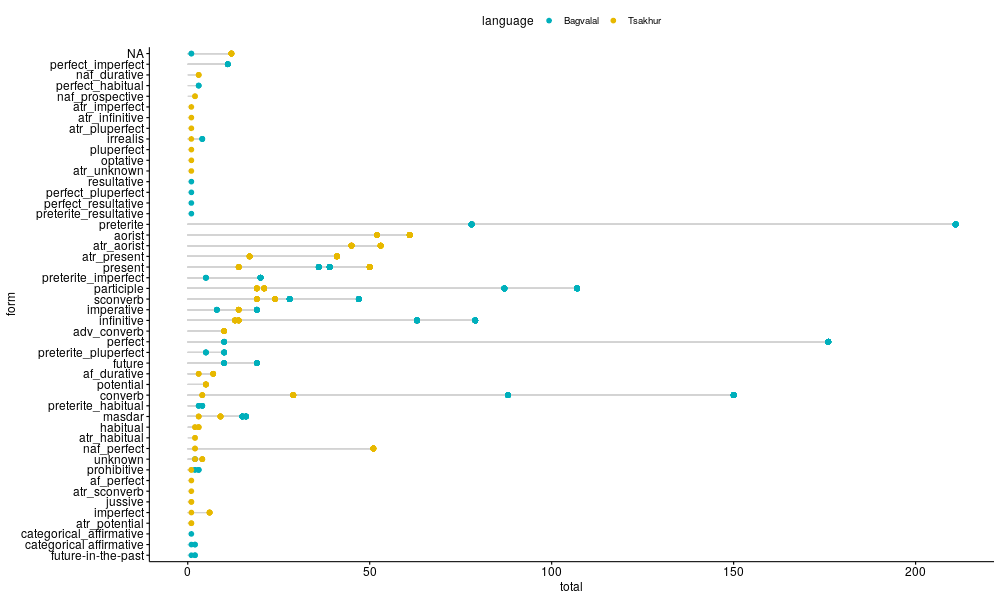
\includegraphics[scale=0.35]{images/forms.png}}
\end{figure}

Если учитывать только клаузы, составляющие главную линию рассказа (тем самым исключая нефинитные клаузы и цитаты), разница сокращается: 14 разных форм в багвалинском языке против 17 в цахурском. Набор используемых форм в нарративных цепочках в целом ограничен, причем можно отметить явное предпочтение общих прошедших и перфектоидов (см. рисунок \ref{fig:forms} и таблицу \ref{tab:narres}).\footnote{Категория <<другие>> в таблице также включает в себя формы так называемых серий, например, туда входит багвалинский Плючквамперфект со вспомогательным глаголом в форме Перфекта.} В целом в цахурском языке используется больше форм иных, чем перфекты, но среди этих других форм самая частотная встречается лишь 46 раз, против 83 перфектоидов.

\begin{table}[H]
\caption{Количество и доля используемых форм в нарративах}
\label{tab:narres}
\vspace{0.2cm}
\begin{center}
\begin{tabular}{lllll}
                                & багвалинский & \% & цахурский & \% \\ \hline
\multicolumn{1}{l|}{прошедшее}  & 244          & 48 & 237       & 58 \\
\multicolumn{1}{l|}{перфектоид} & 171          & 33 & 83        & 20 \\
\multicolumn{1}{l|}{другие}     & 97           & 19 & 89        & 22
\end{tabular}
\end{center}
\end{table}

Рисунки \ref{fig:bagvnar} и \ref{fig:tsakhnar} ниже показывают долю трех категорий форм (прошедшее vs. перфектоид vs. другие) в отдельных нарративах. Судя по количеству зеленого в столбцах на рисунке \ref{fig:bagvnar}, можно предположить, что нарративы 3--5, 8, 10--21, 23--25, 41, 43 и 47 на багвалинском языке являются незасвидетельствованными, поскольку соответствующие им столбцы либо полностью зеленые, либо зеленой является их большая часть. Это предсказание подтверждается для всех текстов кроме текста 47, особенности которого обсуждаются более подробно в разделе \ref{sec:resultsindirect}.

\begin{figure}[H]
\centering
\caption{Формы, используемые в багвалинских нарративных цепочках}
\label{fig:bagvnar}
\vspace{0.5cm}
\fbox{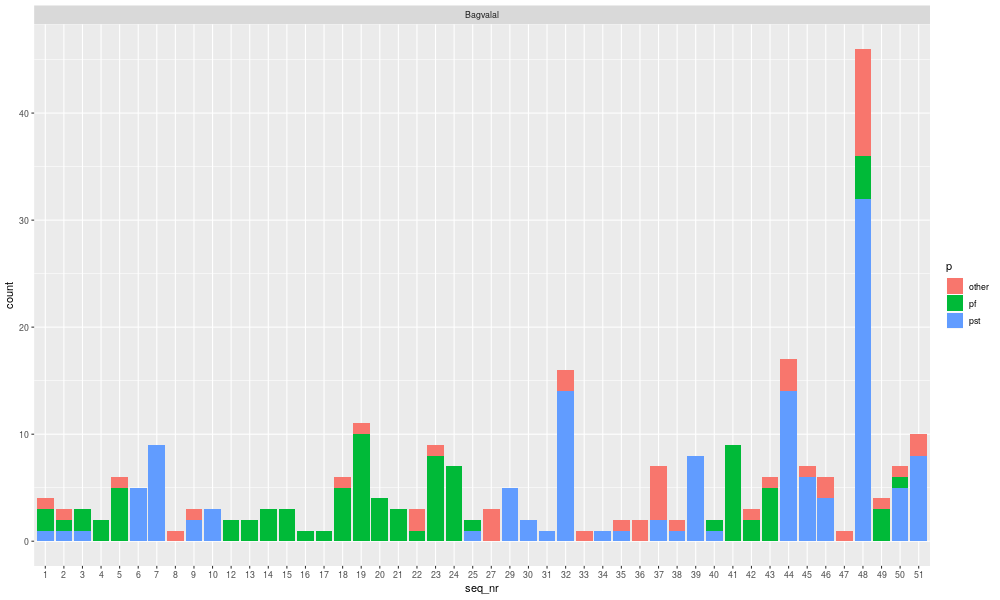
\includegraphics[scale=0.35]{images/bagvbar.png}}
\end{figure}

\begin{figure}[H]
\centering
\caption{Формы, используемые в цахурских нарративных цепочках}
\label{fig:tsakhnar}
\vspace{0.5cm}
\fbox{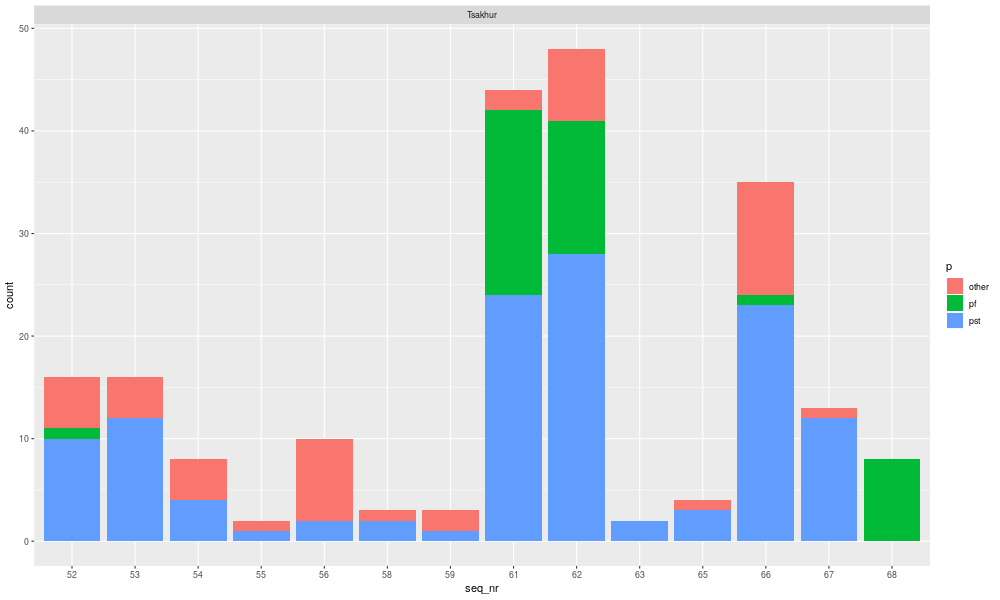
\includegraphics[scale=0.35]{images/tsakhbar.png}}
\end{figure}

В цахурском языке только один текст (68) рассказан полностью в Перфекте. Кроме этого, есть два текста, в которых используется относительно много Перфектов (61 -- 62). В разделах \ref{sec:resultsindirect} -- \ref{sec:resultsdirect} мы обсудим оформление нарративов по отношению к эвиденциальной перспективе, обращая внимание на некоторые неожиданные употребления, а в разделе \ref{sec:statistics} определим статистическую значимость параметра засвидетельствованности для распределения глагольных форм.

\subsection{Незасвидетельствованные нарративы} \label{sec:resultsindirect}

В предыдущем разделе мы заметили, что исходя из рис. \ref{fig:bagvnar} можно предположить, какие из цепочек на багвалинском языке описывают события, незасвидетельствованные говорящим. В следующих цепочках Перфект используется исключительно или преимущественно: 3--5, 8, 10--21, 23--25, 41, 43 и 47. Среди этих 22 цепочек --- 9 полных текстов, и 13 фрагментов (из которых 4 минимальной длины, т.е. две клаузы). Все кроме одного действительно передают события, при которых говорящий сам не присутствовал, включая одну сказку, местные легенды, анекдот, и анекдоты о знакомых людях. На рисунке \ref{fig:bagvnar}, нарратив 47 выглядит как короткий нарратив, который состоит исключительно из Перфектов. Он действительно короткий (предложений всего два), и Перфект в нем только один. Первое предложение возглавляет причастие, а второе — Перфект. В разделе \ref{sec:narseq} мы определили, что нарративная цепочка как состояющую минимум из двух финитных клауз, однако дело в том, что в данном случае причастие в первом предложении на наш взгляд используется в роли сказуемого, см. пример (\ref{ex:turncar1}) и его продолжение в (\ref{ex:turncar2}).

\lb{ex:turncar1}{\gll ce-b muχtar-la mašina-ɬi rek'ʷ-ẽː-w-o, ɬ-oː-b-q'aɬːani jaš-i-la haː-n-o miq'-a-la o-ru-χ w-ič'-inaː-χ-la w-uk'a-w-o mašina \textbf{q'ʷar-oː-b}\\
один-{\N} Мухтар-{\La} машина-{\Inter} садиться-{\Caus}-{\M}-{\Cvb} ехать.{\Ipfv}-{\Ptcp}-{\N}-{\Temp} девушка-{\Pl}-{\La} видеть-{\Hpl}-{\Cvb} дорога-{\Obl}-{\Sup} этот.{\Obl}.{\Hpl}-{\Ad} {\M}-смотреть-{\Ipfv}-{\Cvb}-{\La} {\M}-быть-{\M}-{\Cvb} машина переворачиваться-{\Caus}.{\Ptcp}-{\N}\\
\trans `Когда (мы) однажды, посадив Мухатара в машину, ехали, (Ибрагим,) по дороге увидев девчат и засмотревшись на них, машину \textbf{перевернул}.' \hfill \footnotesize{багвалинский язык\\ \hfill \citep[~760]{bagvalalgram}}}

\lb{ex:turncar2}{\gll heː jaš-i-la esebaː b-eː-r-o, o-ru-r kumuk-la džeː-b-o, mašina \textbf{b-iʁ-eː-b-o} \textbf{ek'ʷa}\\
потом девушка-{\Pl}-{\La} рядом.{\Lat} {\Hpl}-приходить-{\Hpl}-{\Cvb} этот-{\Obl}.{\Hpl}-{\Erg} помощь-{\La} делать-{\N}-{\Cvb} машина {\N}-стоять-{\Caus}-{\N}-{\Cvb} есть\\
\trans `Затем подошли девчата, и с их помощью [=они помощь сделав] \textbf{подняли} машину'\hfill \footnotesize{багвалинский язык\\ \citep[~760--761]{bagvalalgram}}}

Поскольку говорящий, с одной стороны, сам участвовал в ситуации и тем не менее не возникает эффект первого лица (т.е., говорящий будто участвовал неосознанно), заглазное прочтение в этом случае исключено. История является частью разговора, в котором два носителя сначала думают, о чем рассказывать, а потом начинают вспоминать истории про одного родственника. Рассказ в примерах (\ref{ex:turncar1}) -- (\ref{ex:turncar2}) --- первый рассказ, после чего другой носитель рассказывает историю подлиннее. Есть возможность, что первый говорящий своей короткой историей не совсем перешел в нарративный режим, а предложение в (\ref{ex:turncar2}) на самом деле не составляет часть нарратива, а передает релевантный на момент речи факт, что они машину все-таки подняли (с помощью девчат). Без работы с носителями кванадинского диалекта багвалинского языка трудно сказать что-то более определенное. Хотя наличие большого количества Пефректов в багвалинском языке оказывается достаточно надежным индикатором того, что говорящий сам не участвовал в рассказываемых событиях, в текстах имеется 9 незасвидетельствованных нарративов, которые не рассказаны преимущественно в Перфекте. Среди них в том числе сказка, анекдоты про знакомых и местные легенды. Более подробное рассмотрение этих случаев показывает, что в 49-м нарративе все-таки больше Перфектов, чем других форм, а рисунок \ref{fig:bagvindir} показывает, что главная альтернативная стратегия --- с прошедшим / Претеритом. 

\begin{figure}[h]
\centering
\caption{Конкуренция стратегий в незасвидетельствованных нарративах в багвалинском языке}
\label{fig:bagvindir}
\vspace{0.5cm}
\fbox{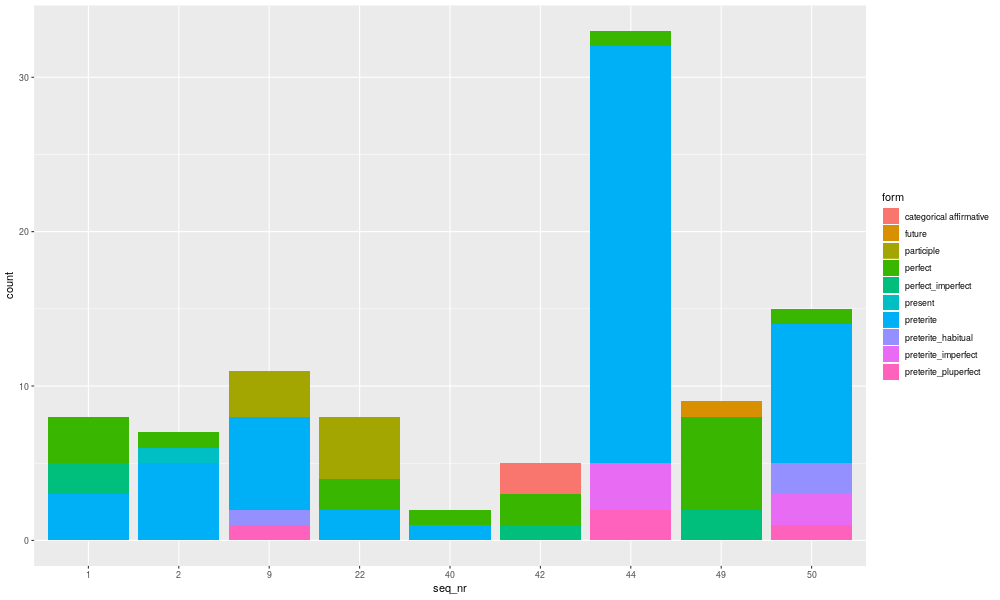
\includegraphics[scale=0.35]{images/bagvalt.png}}
\end{figure}

Интересный случай представляет короткая история 22 о том, как в девятнадцатом веке на селение Кванада напали хуштадинцы --- жители другого багвалинского села --- когда большая часть кванадинской молодежи погибла в Грузии, куда они ездили на разбой. В итоге кванадинцы были вынуждены некоторое время платить налоги хуштадинцам. Эта история в данных была помечена как местная легенда --- говорящий сам не был свидетелем этих событий, и рассказывает про события в очень общих чертах. Основная линия этой истории оформлена причастиями --- стратегия, которая требует дальнейшего изучения. Напоминаем, что в аварском языке раньше тоже существовала нарративная стратегия с причастиями прошедшего времени, имевшая эвиденциальное или модальное значение (см. раздел \ref{sec:ndevid}).
\par В цахурских текстах имеется только один рассказ (68), который полностью рассказан в Перфекте. Это анекдот о том, как сывагильцы ловили медведя. В этом анекдоте жители селения Сывагиль (цахурское селение в Азербайджане) идут ловить медведя. Когда медведь их увидел, он убежал в берлогу, после чего сывагильцы засунули одного человека в берлогу. Когда его оттуда вытащили, он оказался без головы. Сывагильцы начали спорить, была ли у него голова раньше, до того, как они засунули его в берлогу. В конце истории они спрашивают у его жены — была ли у ее мужа голова, на что она отвечает, что не уверена, что голова была --- помнит только, как у него усы двигались, когда он ел хинкал. Поскольку этот сюжет фиктивный, его можно отнести к анекдотам. Единственная сказка в цахурском материале (67) рассказана в Аористе.\footnote{Сюжет тоже представлен в сборнике даргинского фольклора \citep[114--116]{vandenberg2001}, только в той версии, главные персонажи просто трое друзей, без местной специфики, и жена человека без головы помнит только как он каждый год купил новую шляпу. В \citep{tsakhurgram} приводится следующее примечание по поводу него: <<Приводимый ``бродячий'' сюжет широко засвидетельствован в фольклоре различных народов, ср. тот же анекдот (``Догада''), записанный в верховье Мезени в 1916 г. и приведенный в сборнике сказок русского Севера (Озаровская 1931, с. 403--404).>>}
\par Нарративы 61 и 62, в которых чередуются Аористы и (неатрибутивные, то есть эпистемические) Перфекты, записаны от одного и того же носителя, который рассказывает истории про известных местных людей (вор в законе Ибрагим-паша и конокрад Темраз). Пересказы не привязаны к определенному первичному источнику, например, в конце (61), говорящий заключает историю замечанием: <<Вот такую историю люди про него рассказывают>>. В случае нарратива 62, нам осталось не до конца понятным, ведет ли говорящий рассказ, опираясь на собственный опыт, или нет. В итоге мы считаем, что в цахурском материале есть четыре рассказа о незасвидетельствованных событиях: 62 про Ибрагим-паши, 67 --- сказка, 68 --- анекдот про Сывагильцев и 53 --- короткая легенда про предателя Саида, который оказался не предателем. Последний рассказан в Аористе.

\subsection{Засвидетельствованные нарративы} \label{sec:resultsdirect}

В засвидетельствованных нарративах встречаются преимущественно простые прошедшие. В багвалинском языке стратегия отличается только в нарративах 27 и 37: оба они из диалога про поездку с лингвистами во время экспедиции. В нарративе 27 преобладает причастие, а в 37 --- настоящее время, используемое как praesens historicum. Стратегия с настоящим временем также представлена в одном цахурском тексте. Остается неизвестным, возможна ли такая стратегия при рассказе о незасвидетельствованных событиях, или она характерна именно для рассказов из собственного опыта. Перфект в засвидетельствованных нарративах встречается всего 9 раз: 3 в цахурском (один атрибутивный, два неатрибутивных) и 6 в багвалинском. Один из этих случаев (про перевернутую машину) уже упоминался в разделе \ref{sec:resultsindirect}. 
\par В рассказе 48, говорящий рассказывает про то, как они с родственником на грузовике спускались из села и поехали в Ставропольский край, везя в кузове вещи и пассажиров в кузове. Пока они спускались по плохим дорогам, в кузове происходили разные события, о чем водителю и говорящему было неизвестно. Они узнали об этих событиях только потом, и именно эта информация рассказана в Перфекте, или с конструкцией с глаголом ‘найти’, тогда как основная линия рассказа ведется в Претерите. В цахурских текстах неатрибутивный Перфект используется в короткой истории о том, как друг говорящего в молодости притворялся, что он сломал ногу, чтобы не пойти в магазин (52). История рассказана в основном в Аористе, но Перфект используется, когда говорящий рассказывает о том, что они с друзьями только потом узнали, что и почему сделал этот человек.

\vfill
\pagebreak

\lb{ex:leg}{\gll χɨliːdže sem-mɨ a-t’-k’ɨn-iː-l-e qiːʁa ša-k’le ac’a-xa-jn-ki maˁhammad-ɨ-s \textbf{d-ɨkːiːkɨn-o-r} magazinɣ-eː-qa		ajr-es hamančiše \textbf{aˁmal-bɨ} \textbf{wo-d} \textbf{haʔ-u} ɢelj ha-t’-q’ur-wɨ\\
спустя год-{\Pl} {\Npl}-уходить.{\Pf}-{\Msd}-{\Sup}-{\El} после мы.{\Obl}-{\Aff} знать-{\Iv}.стать.{\Pf}-{\Atr}-{\Ki} Магомед-{\Obl}-{\Dat} {\Neg}-хотеть.{\Pf}-быть={\First} магазин-{\In}-{\All} {\M}.приходить-{\Pot} поэтому хитрость-{\Pl} быть-{\Npl} делать-{\Pf} нога.{\Iv} {\Iv}-ломать.{\Pf}-{\Wy}\\
`Через [=спустя] много лет мы узнали, что Магомед \textbf{не хотел} идти в магазин и поэтому \textbf{притворился}, что сломал ногу.' \\ \footnotesize{\citep[~757--758]{tsakhurgram} \hfill цахурский язык}}

\subsection{Другие нарративные стратегии} \label{sec:resultsotherstrat}

В одном багвалинском тексте говорящий пересказывает анекдот про своего знакомого, где он после первого предложения переходит на перспективу первого лица и рассказывает всю историю как бы от имени главного персонажа, см. первые два предложения анекдота в примерах (\ref{ex:firstp1})--(\ref{ex:firstp2}).\footnote{В разделе \ref{sec:methodanalysis} мы обсуждали подобную стратегию в нарративе из рикванинского диалекта андийского языка, где говорящий пересказывал историю своего деда.}

\lb{ex:firstp1}{\gll o-šːu-r b-as-in-oː-b b-uk’a e-w grozni-la ek’ʷa-b-q’arɬːir in-šːu-r j-ihi-ʁala čačana-j\\
этот-{\Obl}.{\M}-{\Erg} {\N}-рассказывать-{\Ipfv}-{\Ptcp}-{\N} {\N}-быть {\Log}-{\M} Грозный-{\Loc} есть-{\Ptcp}.{\N}-{\Temp} {\Log}-{\Obl}.{\M}-{\Erg} {\F}-брать={\Rala} чеченка-{\F}\\
\trans `Он рассказывал, что когда он был в Грозном, женился на чеченке.' \\ \footnotesize{\citep[787]{maisaktatevosov2007} \hfill багвалинский язык}}

\lb{ex:firstp2}{\gll o-j haddiɬir j-uχːu-č’i \textbf{di-č’}\\
этот-{\F} долго {\F}-оставаться-{\Neg} я.{\Obl}-{\Cont}\\
\trans `Она долго \textbf{у меня} не осталась.' \\ \footnotesize{\citep[787]{bagvalalgram} \hfill багвалинский язык}}

Стратегии непрямого нарратива с репортативной частицей в багвалинском и цахурском языках не представлены. В цахурском языке подобного рода частицы отсутствуют, а семантически похожие частицы эпистемического статуса не используются в главной линии, как уже обсуждалось в разделе \ref{sec:samplelanguages}. В багвалинском языке имеются квотативы, которые иногда употребляются в качестве репортатива, но нарративная стратегия с квотативными частицами в репортативной функции отсутствует. Багвалинская конструкция с `найти' используется только в тех эпизодах внутри рассказа, которые описывают ситуацию непосредственного обнаружения, ср. Текст 8, предложения 88--92 \citep[771]{bagvalalgram}.

%неясные случаи цахурской выборки

\subsection{Статистическая значимость засвидетельствованности как параметра} \label{sec:statistics}

В целом оба языка показывают распределение, похожее на андийские данные, представленные в разделе \ref{sec:andinarr}. Перфектоиды значительно более распространены в контекстах, где говорящий рассказывает не о собственном опыте, хотя в цахурских данных этот эффект возникает в основном благодаря вкладу одного носителя (см. раздел \ref{sec:resultsindirect}). В контексте прямой засвидетельствованности преобладает общее прошедшее. Отношения при этом не симметричные ---  общие прошедшие используются также в контексте косвенной засвидетельствованности, а перфектоиды почти полностью отсутствуют в контексте прямой засвидетельствованности. При этом цахурский Аорист в незасвидетельствованных контекстах более частотен, чем Перфект, тогда как в багвалинском языке Перфект преобладает над Претеритом в заглазном контексте.

\begin{table}[h]
\caption{Перфектоиды и прошедшие в багвалинских и цахурских нарративах согласно перспективе свидетельства}
\label{tab:conting}
\vspace{0.2cm}
\begin{center}
\begin{tabular}{lllll}
                                & \multicolumn{2}{c}{багвалинский} & \multicolumn{2}{c}{цахурский} \\ \cline{2-5} 
                                & прям.           & косв.          & прям.         & косв.         \\ \hline
\multicolumn{1}{l|}{перфектоид} & 6               & 165            & 3             & 50            \\
\multicolumn{1}{l|}{прошедшее}  & 181             & 63             & 79            & 86           
\end{tabular}
\end{center}
\end{table}

%Двусторонний точный тест Фишера подтверждает, что наблюдаемая корреляция между употреблением форм и перспективой свидетельства — статистически значима для обоих языков, со значениями p намного ниже 0.05 (< 2.2e-16 для багвалинских данных, и 3.204e-09 для цахурских).

% ФИШЕР / ХИ-КВАДРАТ ПРО ЯЗЫК — НЕЗАСВ.

Тест хи-квадрата подтверждает, что наблюдаемая корреляция между употреблением форм и перспективой свидетельства — статистически значима для обоих языков, со значениями p намного ниже 0.05 (\textless 2.2e-16 для багвалинских данных, и 8.463e-08 для цахурских, в обоих случаях степень свободы была 1). 

\section{Итоги} \label{sec:itogi3}

Известно, что в языках с эвиденциальным перфектоидом эта форма часто выступает в рассказах о незасвидетельствованных событиях. Наоборот, в языках, где косвенная засвидетельствованность как значение перфектоида отсутствует, перфектоид часто практически не используется в главной линии нарратива, за исключением выделения определенного события в контекстах с семантикой текущей релевантности (раздел \ref{sec:intro3}). В настоящей главе мы более подробно проанализировали нарративный режим речи носителей исследуемых языков. В простых, элицитированных нарративах на разных диалектах андийского языка, в котором перфектоид может иметь значения результатива, текущей релевантности и косвенной засвидетельствованности, форма может употребляться для главной линии рассказа о незасвидетельствованных событиях, но также для обозначения неожиданных событий внутри рассказа в Аористе (см. раздел \ref{sec:andinarr}). Такую стратегию оформления нарратива о незасвидетельствованных событиях мы назвали перфектоидной. Перфектоидная стратегия используется не всегда и не всеми носителями. Встречается и использование Аористной стратегии, появляющейся вне зависимости от эвиденциальной перспективы, причем в случае нарратива о незасвидетельствованных событиях факультативно можно использовать репортативную частицу. Данные элицитированных нарративов противоречат данным, полученным элицитацией анкеты. Если судить по результатам анкетирования, в рикванинском диалекте эвиденциальное значение более грамматикализовано, чем в зиловском (см. раздел \ref{sec:elicitation}). Однако при элицитации нарративов только 1 из 5 рикванинских носителей использовал перфектоидную стратегию в незасвидетельствованном контексте, в то время как из 6 носителей зиловского диалекта перфектоидную стратегию использовали 5 носителей (раздел \ref{sec:andinarr}). Методологическая проблема заключается в том, что вариативность, наблюдаемая при элицитации, может быть результатом не только особенностей речи определенных носителей или групп носителей, но и разных условий эксперимента (например, сосредоточенность носителя или поведение исследователя. С другой стороны, эти данные теоретически могут свидетельствовать об особом статусе использования перфектоида именно в нарративе --- в частности, о возможности заимствования перфектоидной стратегии нарратива как способа грамматического оформления определенного типа дискурса вне зависимости от степени грамматикализованности у перфектоида эвиденциального значения.
\par Для того, чтобы подтвердить или опровергнуть эти предположения, в разделе \ref{sec:results} мы рассмотрели естественные нарративы на двух языках с разными функциональными профилями перфектоидов: багвалинском и цахурском. В обоих языках перфектоиды ассоциируются с заглазностью, но в случае цахурского языка косвенная засвидетельствованность не считается главной функцией этой формы, а лишь контекстной импликатурой, часто возникающей в связи с тем, что форма выражает дистанцирование говорящего от описываемой ситуации (ее предположительная основная функция). Подобные идеи о семантике перфектоидных форм с эвиденциальным уклоном встречаются также у исследователей других языков эвиденциального пояса (см. раздел \ref{sec:pftyp}). По нашим данным, перфектоид в обоих языках значительно более частотен в незасвидетельствованном контексте (раздел \ref{sec:resultsindirect}), чем в контекстах прямой засвидетельствованности (\ref{sec:resultsdirect}), хотя и в цахурском, и в багвалинском языках использование общего прошедшего остается возможным и в заглазных нарративах. При этом в цахурском языке даже в незасвидетельствованном нарративе Аорист более частотен, чем Перфект, в то время как в багвалинском языке Перфект в незасвидетельствованных нарративах преобладает. Эта разница между багвалинским и цахурским в плане относительной частотности простого прошедшего и перфектоида в заглазных нарративах в принципе подтверждает существующую интерпретацию перфектоидов в этих языках: багвалинский перфектоид более, а цахурский --- менее эвиденциален, следовательно простое прошедшее в цахурском языке --- более нейтральный нарративный выбор, а в багвалинском - наоборот, менее нейтральный. Поскольку мы нам была доступна лишь небольшая выборка текстов, этот результат требует подтверждения.
\par Таким образом, мы предпологаем, что использование перфектоидов в (заглазном) нарративе может служить объективной сопоставительной мерой степени его грамматикализованности, в противовес анализу, базирующемуся на сравнении элицитированных анкет. С другой стороны, тот факт, что употребление перфектоида в главной линии заглазных нарративов представлено в разных языках и идиомах, включая и те, где эвиденциальная семантика не очень ярко ощущается носителями (например, в зиловском андийском), или те, в которых форма используется скорее для обозначения более абстрактной дистанции (в цахурском), в принципе может указывать и на то, что данное употребление является в какой-то степени независимым свойством перфектоидов. В разделе \ref{sec:pftyp} мы обсуждали следующий путь развития заглазных употреблений перфектоидов: сначала инферентивное значение возникает как дискурсивная импликатура, затем форма может расширить свой контекст употребления на ситуации, где говорящий не видел даже результата или последствия события, о котором он рассказывает, а имеет какие-то другие косвенные сведения о нем, например, знает о нем с чужих слов. На данном этапе становится возможным использовать форму для оформления заглазных нарративов, включая не только такие традиционные жанры как сказки и легенды, но более реальные истории, при которых говорящий не присутствовал.
\par Можно представить себе сценарий, при котором такое употребление заимствуется из контактного языка в качестве стилистического приема, без наращения эвиденциальной семантики в других контекстах. Однако по нашим данным нарративное употребление отсутствует в тех языках, где перфектоид в других контекстах вообще не имеет эвиденциальной функции, как в рутульском и лезгинском (за исключением более или менее редких инферентивных импликатур, отмечаемых, например, для лезгинского), см. \ref{tab:svod}. В зиловском диалекте андийского языка, для которого мы зафиксировали только нарративное употребление перфектоида, нарратив служит <<хранителем>> эвиденциальной категории, которая в обычной речи утрачивается или по крайней мере (согласно интуиции носителей данного диалекта по сравнению с носителями других диалектов андийского) менее ярко выражена. Можно сделать следующий вывод: для того, чтобы форма могла приобрести нарративную функцию передачи заглазности, инферентивное или эвиденциальное ядро уже должно иметь место в других контекстах. При этом мы считаем вполне вероятным, что нарративное употребление эвиденциального перфектоида в одном языке по крайней мере может способствовать появлению такого же употребления в другом языке, который находится в контакте с первым.
\par Как мы уже отметили --- гипотеза о появлении эвиденциального значения перфектоида под влиянием контакта с тюркскими языками труднодоказуема, во-первых, в отсутствие достаточных исторических данных о самих языках и языковых контактах и, во-вторых, в связи с тем, что инферентивная импликатура перфектоидных форм является естественной и распространенной вне зависимости от принадлежности языка определенному ареалу (\ref{sec:pftyp}).\footnote{Как обсуждалось в разделе \ref{sec:itogi2}, реконструкция контактного сценария еще более затруднена тем, что нахско-дагестанские перфектоиды в формальном плане не очень похожи на их тюркские эквиваленты.} Заглазные перфектоиды представлены и вне ареала <<эвиденциального пояса>>, хотя в его границах они встречаются чаще. В связи с этим Л. Йохансон замечает, что контакты носителей кавказских языков с тюркскими языками, вероятно, лишь усиливали тенденции к развитию заглазного значения, уже присутствующие в самих языках-реципиентах \citep[172]{johanson2006}. Мы выдвигаем гипотезу о том, как  именно эвиденциальные компоненты значения формы могут усиливаться в ситуации языкового контакта через нарративные употребления.
\par Нарративное употребление играет важную роль при освоении категории эвиденциальности в детской речи. В речи турецких родителей прошедшее заглазное часто употребляется при общении с детьми в контексте нарративов о выдуманных событиях, которые по определению являются незасвидетельствованными \citep{aksu88}. Таким образом дети знакомятся с заглазной функцией этой формы прошедшего времени (видовое значение --- указание на стативную ситуацию --- они осваивают еще до этого) (ibid.). В детской речи эвиденциальное употребление впервые появляется в сказочных формулах, таких как «было, не было» (ср. раздел \ref{sec:ndlang}). На данном этапе употребление формы по-видимому еще не имеет семантического наполнения - дети просто повторяют употребление за взрослыми, не осознавая, какую функцию в данном случае несет заглазное прошедшее (форма на \textit{-mIš} в турецком языке) \citep{aksu2009}.\footnote{Интересно отметить, что в удинском языке распространенная сказочная формула <<было, не было>> по примеру азербайджанского языка используется в форме перфекта, так же как и в турецком языке \citep{maisak2018}. При этом для удинского перфектоида и его азербайджанского аналога эвиденциальность не характерна. Соответственно, употребление перфекта в нарративе ограничивается формулой и отдельными предложениями --- нарративное употребление как таковое (главная линия рассказа в перфекте) не представлено.} После этого они усваивают значение инферентива, после него --- значение репортатива. Как мы отмечали в разделе \ref{sec:pftyp}, освоение последних двух значений у детей и в других языках, по-видимому, идет параллельно общим тенденциям грамматикализации форм косвенной засвидетельствованности, в которых инферентивное значение предшествует репортативному. Нам представляется возможным, что, аналогично тому, какую роль нарративное употребление играет в турецкой речи, направленной к детям, нарративное употребление в одном языке может стимулировать развитие заглазности в контактирующем языке. 
\par Перфектоид с эвиденциальным значением, который используется в заглазных нарративах, можно рассматривать как своего рода minimally counterintuitive concept (MCI) --- понятие из когнитивной антропологии, которое используется для объяснения широкого распространения определенных религиозных идей \citep{boyer2001}, \citep{barrettnyhof2001}. MCI концепты основаны на знакомых понятиях и категориях, и в большей части соответствуют интуитивным ожиданиям, связанным с этими понятиями, но одновременно нарушают небольшой (minimal) объем этих ожиданий. В качестве примера можно привести понятие <<призрака>>, которое находится в народных верованиях по всему миру. Призрак по сути человек, который может проходить через стены и другие сплошные объекты. Кроме этого последнего <<нарушенного ожидания>>, он соответствует многим предположениям, которые вызывает понятие <<человек>>: у него есть какая-то история, он имеет свои мысли и эмоции, он ищет общения с другими людьми, и так далее, см. \citep{barrettnyhof2001}, \citep{boyer2001}. Широкое распространение таких понятий обусловлено тем, что они опираются на нечто интуитивно понятное, но добавляют туда нечто новое, что делает их запоминающимися \citep[72]{barrettnyhof2001}. Поэтому они запоминаются лучше,
чем понятия, которые полностью соответствуют или, наоборот, сильно нарушают ожидания. Для носителя языка с обычным перфектом, нарративное употребление подобной формы необычно и до какой-то степени противоречит ожиданиям и именно поэтому очень заметно. Такая форма сочетает частичное оправдание ожиданий (она похожа на форму в языке реципиента, например, семантикой результатива или текущей релевантности в сопоставлении с общим прошедшим) с их нарушением (перфектоид используется в нарративной цепочке). Языки, в которых инферентивная импликатура уже достаточно конвенционализирована в этом плане представляют особо плодородную почву для дальнейшего развития заглазной семантики. Такой механизм может объяснить широкое распространение данной <<граммемы>> (грамматическая семантическая единица, ср. ) как своего рода грамматического мема \citep{boyer2001} в условиях интенсивного обмена фольклорными традициями. Нарративное употребление формы в такой ситуации может действовать как <<перцептивный магнит>> (ср. \citep{blevins2017} об этом эффекте в фонологии), который усиливает уже присутствующую склонность к инферентивной/эвиденциальной интерпретации.
\par В случае Восточного Кавказа и прилегающих территорий обмен фольклорными традициями действительно имел место, что проявляется в наличии общих сюжетов и в ареальных паттернах их распространения, ср. \citep{adzhiev1991intro}. Роль такого обмена в эволюции перфектоидов может быть подтверждена или опровергнута масштабным сопоставительным изучением употребления форм в фольклорных и других текстов из данного региона. Возможные пути такого исследования предварительно намечены в работе в виде пилотных микроисследований (разделы \ref{sec:svod}, \ref{sec:results}), но в целом оно пока остается задачей для будущего.

